%% Where Should the Adapter Go? Outlier Dimensions, Rank Allocation and
%% Placement in Low-Rank Adaptation of Small Language Models
%% IEEE conference format (IEEEtran).
\documentclass[conference]{IEEEtran}
\IEEEoverridecommandlockouts

\usepackage{cite}
\usepackage{amsmath}
\usepackage{newtxtext,newtxmath}
\newtheorem{proposition}{Proposition}
% Numbers still to be filled from the result files show up red in the draft.
\newcommand{\NUM}[1]{\textcolor{red}{#1}}
\newcommand{\TODO}[1]{\textcolor{red}{[TODO: #1]}}
\usepackage{algorithm}
\usepackage{algpseudocode}
\usepackage{graphicx}
\usepackage{booktabs}
\usepackage{multirow}
\usepackage{textcomp}
\usepackage{xcolor}
\usepackage{pgfplots}
\pgfplotsset{compat=1.18}
\usepackage[hidelinks]{hyperref}

% The appendix is mostly wide tables; let LaTeX put more than one on a float page
% instead of leaving half-empty pages (round-2 NEW-7).
\renewcommand{\topfraction}{0.92}
\renewcommand{\bottomfraction}{0.7}
\renewcommand{\textfraction}{0.07}
\renewcommand{\floatpagefraction}{0.75}
\setcounter{topnumber}{3}
\setcounter{totalnumber}{5}

\def\BibTeX{{\rm B\kern-.05em{\sc i\kern-.025em b}\kern-.08em
    T\kern-.1667em\lower.7ex\hbox{E}\kern-.125emX}}

\newcommand{\method}{\textsc{Drift}}
\newcommand{\R}{\mathbb{R}}
\newcommand{\E}{\mathbb{E}}
\newcommand{\tr}{\operatorname{tr}}
\DeclareMathOperator*{\argmax}{arg\,max}
\DeclareMathOperator*{\argmin}{arg\,min}

\begin{document}

\title{Where Should the Adapter Go?\\ Outlier Dimensions, Rank Allocation and
Placement in Low-Rank Adaptation of Small Language Models}

%% AUTHOR BLOCK --- fill this in before submission (round-2 item NEW-5).
%% Single-blind / camera-ready: replace the four fields below with your details.
%% Double-blind: comment out the block in use and uncomment the anonymous one,
%% which carries no name, affiliation or e-mail.
\author{\IEEEauthorblockN{Author Name}
\IEEEauthorblockA{\textit{Department} \\
\textit{Institution}\\
City, Country \\
gowhar390275@gmail.com}
}
%% Anonymous alternative for a double-blind venue:
% \author{\IEEEauthorblockN{Anonymous submission}
% \IEEEauthorblockA{Paper ID \textit{nnnn}}
% }

\maketitle

\begin{abstract}
Activation-guided methods such as EVA decide where a low-rank adapter's capacity
goes by profiling the target task's activations beforehand. We test whether this
helps small language models on biomedical classification when budgets are matched
and each configuration's learning rate is tuned on its own dev set. Across
eleven methods on three benchmarks, none beats a tuned uniform LoRA by more than
$0.34$ F1 ($1.0$ under HoC's micro-F1), and no difference survives a
multiple-comparison correction. A budget sweep, a $4$M--$110$M ladder, a decoder
SLM and a clinical task agree once multiple comparisons are corrected ($1{,}328$
runs). The methods differ in stability instead, and for activation-PCA
initialisation we can trace the cause. On RoBERTa-base, its leading directions
lie on the backbone's outlier dimensions 77 and 588 at 23--24 of the 24 distinct
hidden-state inputs and carry a median $59$--$73\times$ an average direction's
energy, and budget-matched EVA loses 2 of 5 HoC seeds in fp16 and all 3 in fp32.
The decoder's signature is even stronger. Whitening these directions, deflating a
general-domain reference subspace (\method{}, which nests EVA) or the exact
generalised-eigenvector contrast all largely restore stability (whitening most
reliably) but add no accuracy we can detect at this power. A random-token
reference serves as well as real text, so the reference supplies the backbone's
outliers, not domain knowledge. Neither rank allocation nor placement helps at a
matched budget, and halving the budget costs nothing. Where a larger budget
helps, allocation still does not. We close with a protocol for evaluating
allocation.
\end{abstract}

\begin{IEEEkeywords}
parameter-efficient fine-tuning, low-rank adaptation, small language models,
outlier dimensions, domain adaptation, biomedical text classification
\end{IEEEkeywords}

\section{Introduction}

Text classification in specialised domains, such as clinical triage,
pharmacovigilance and literature curation, is increasingly deployed under
constraints that rule out large models. Patient data cannot leave the
institution, inference must run on commodity hardware, and dozens of
task-specific classifiers must be served concurrently. Small language models
(SLMs), from a few million to a few hundred million parameters, suit this
setting well, and parameter-efficient fine-tuning (PEFT) is the natural way to
specialise them. A frozen backbone is shared across tasks, while a small
adapter, typically well under $1\%$ of the parameters, carries the task-specific
update~\cite{hu2022lora,han2024peftsurvey}.

This raises a question that is simple to state but matters more than it might
seem: \emph{given a fixed adapter budget, where in the network should the
capacity go?} Uniform allocation, as in standard LoRA~\cite{hu2022lora}, is
budget-oblivious, so a productive line of work allocates rank non-uniformly.
One family does this \emph{during} training, pruning or growing ranks by
importance scores~\cite{zhang2023adalora,ding2023sora,valipour2023dylora}. A
second, faster family does it \emph{before} training, by profiling activation geometry on a
small calibration set. EVA initialises adapters from the principal directions of
the target activations and redistributes rank by explained
variance~\cite{paischer2025eva}. CorDA~\cite{yang2024corda} and
AIRA~\cite{li2025aira} weight the weight-matrix SVD by an activation
covariance, and TLoRA~\cite{lin2026tlora} and Liu et al.~\cite{liu2026rsprobe}
score layers by task sensitivity or effective rank.

Whether such allocation helps depends on how it is compared. Methods differ in
the learning rates they favour, so a baseline that borrows the new method's
learning rate is not a neutral reference. Moving rank between modules of
different width also changes the number of parameters spent, which means that a
matched rank is not a matched budget. Lee et al.~\cite{lee2026lrmatters}
recently showed that LoRA and nine of its variants reach similar peak
performance on decoder LLMs once the learning rate of every method is tuned.
Training-free allocation has not been evaluated under the same protocol, and
neither has the regime in which a good allocation should matter most, namely
small backbones adapted to a specialised domain.

In domain adaptation the question takes a sharper form. Biomedical text is still
English. Its dominant activation directions are largely those of general text,
which the pretrained model already handles, so profiling a single distribution
may spend capacity where none is needed. If allocation is to help, it should
target directions that carry substantial target-domain energy \emph{and} are
poorly represented in pretraining, and only a contrast between two distributions
can reveal such directions. To give activation-guided allocation its best
chance, we build that contrast into an instrument rather than a competing
method. \method{} (Domain-Residual Informed Fine-Tuning) deflates the target
activation covariance by the principal subspace of a general-domain reference
corpus, allocates a global parameter budget over the resulting \emph{drift}
spectrum, and initialises each adapter inside the residual subspace. It needs
two forward passes and no labels or gradients. Its deflation level $\tau$
contains EVA as the special case $\tau = 0$, which isolates the effect of the
contrast from everything else, and its exact counterpart, the generalised
eigenvectors of the target and reference covariances, tests the contrast in its
principled form.

Allocation should matter most for small models. Aghajanyan et
al.~\cite{aghajanyan2021intrinsic} show that the intrinsic dimension of
fine-tuning \emph{grows} as models shrink. A smaller backbone therefore needs a
higher-rank update to reach the same quality, and so has less slack to absorb a
misallocated budget. This predicts that careful allocation should pay off more
as the backbone gets smaller, and we test the prediction on a controlled
parameter ladder. The study is organised around four questions:
\begin{itemize}
\item[\textbf{RQ1}] Under matched parameter budgets, with every configuration
      tuned on its own, does any allocation or initialisation scheme beat
      uniform LoRA?
\item[\textbf{RQ2}] Why is activation-PCA initialisation fragile, and does
      removing the cause help?
\item[\textbf{RQ3}] Which design choice matters (rank allocation,
      initialisation or placement), and does placement still matter when the
      budgets are matched?
\item[\textbf{RQ4}] Does the answer change with the backbone's size or
      architecture?
\end{itemize}

\noindent\textbf{Findings.} This is an evaluation study, and its contributions
lie in its findings:
\begin{itemize}
\item \emph{RQ1:} under matched budgets and per-configuration tuning, no method
      beats LoRA by more than $0.34$ F1, no difference with LoRA survives a
      Holm correction, and the methods differ in stability rather than
      accuracy (Section~\ref{sec:main}).
\item \emph{RQ2:} on RoBERTa-base, the leading directions of activation PCA lie
      on the backbone's known outlier dimensions and carry tens to thousands of
      times the energy of an average direction. Recurring dimensions play the
      same role in BERT-Base, BERT-Medium and a decoder SLM. Whitening,
      reference deflation and the generalised eigenvectors form one family of
      remedies. All of them restore most of the stability, none turns it into
      accuracy, and the reference corpus matters only through the backbone's
      outlier dimensions, since random tokens serve as well as WikiText
      (Sections~\ref{sec:outliers} and~\ref{sec:scale}).
\item \emph{RQ3:} rank allocation alone slightly hurts, and a stable
      data-derived initialisation helps at most marginally
      (Section~\ref{sec:ablation}). Adapter placement produces no reliable
      change at a matched budget either. The feed-forward advantage reported by
      He et al.~\cite{he2022unified} does not appear under our controls, and
      all-module LoRA at half the budget matches the full budget on every task
      (Section~\ref{sec:placement}).
\item \emph{RQ4:} with every method tuned on each backbone, no gain over LoRA
      on the BERT ladder survives correction. EVA's large deficit on small
      backbones at a rate tuned for RoBERTa-base shrinks to at most $2.5$
      points at its own rate. The decoder SmolLM2-360M has the strongest
      outlier signature and repeats the pattern seen on RoBERTa
      (Section~\ref{sec:scale}), and so do clinical notes
      (Section~\ref{sec:clinical}).
\end{itemize}
Along the way, we provide \method{}, a training-free two-distribution profiler
that nests EVA and isolates the contrast (Section~\ref{sec:method}), and a
protocol for evaluating adapter allocation (Section~\ref{sec:discussion}).

\section{Related Work}

\noindent\textbf{Parameter-efficient fine-tuning.}
Adapter bottlenecks~\cite{houlsby2019adapters}, prompt and prefix
tuning~\cite{lester2021prompt,li2021prefix}, sparse bias
tuning~\cite{benzaken2022bitfit} and rescaling
vectors~\cite{liu2022ia3} all restrict the update to a small subspace.
LoRA~\cite{hu2022lora} is the dominant variant because its update merges into
the base weights and leaves the inference cost unchanged. DoRA~\cite{liu2024dora}
decomposes the update into magnitude and direction, VeRA~\cite{kopiczko2024vera}
shares random projections across layers, and QLoRA~\cite{dettmers2023qlora}
combines LoRA with quantisation.

\noindent\textbf{Careful re-evaluation.}
Lee et al.~\cite{lee2026lrmatters} re-evaluate nine LoRA variants with a
separate learning-rate search for each method. They find that all reach similar
peak performance on decoder LLMs and trace the differences in their optimal
learning rates to the largest eigenvalue of the loss Hessian. Biderman
et al.~\cite{biderman2024lorlearnsless} document the accuracy gap that remains
between LoRA and full fine-tuning, particularly in domains far from pretraining,
which is the regime we target. We extend the first kind of study to
training-free rank allocation, matched parameter budgets and small encoders, and
we add a mechanistic account of the failure we observe.

\noindent\textbf{Rank allocation.}
AdaLoRA~\cite{zhang2023adalora} parameterises the update in SVD form and prunes
singular triplets by a sensitivity score during training.
SoRA~\cite{ding2023sora} gates ranks with a sparsifying penalty, and
DyLoRA~\cite{valipour2023dylora} trains nested ranks. These methods require a
training run and start from an inflated budget. Training-free allocation is more
recent. EVA~\cite{paischer2025eva} redistributes rank by explained variance
ratio, AIRA~\cite{li2025aira} by layer-wise outlier ratios,
TLoRA~\cite{lin2026tlora} by a sensitivity metric over $W\Sigma_x$, and Liu et
al.~\cite{liu2026rsprobe} by effective rank plus a Fr\'echet distance
under virtual perturbation. All of them use statistics of the target task alone.
CorDA~\cite{yang2024corda}, in its knowledge-preserving mode, uses a covariance
from a second distribution to decide which components to freeze, but to our
knowledge \method{} is the first to \emph{allocate rank} by a contrast between two
distributions.

\noindent\textbf{Spectral initialisation.}
PiSSA~\cite{meng2024pissa} initialises the adapter from the leading singular
directions of $W$ and trains those, MiLoRA~\cite{wang2025milora} uses the
trailing ones, and LoRA-GA~\cite{wang2024loraga} aligns the initialisation with
the first task gradient. CorDA~\cite{yang2024corda} orients the decomposition of
$W$ using an input-activation covariance. Unlike these methods, \method{}
decomposes the \emph{difference in input geometry} between two corpora, not the
weight matrix.

\noindent\textbf{Where and at what scale to adapt.}
The question of which matrices to adapt goes back to LoRA itself, whose authors
compare subsets of the attention projections at a fixed parameter
count~\cite[Sec.~7.1]{hu2022lora}. He et al.~\cite{he2022unified} find that
modifying feed-forward representations uses added parameters more effectively
than modifying attention, although attention-only prefix tuning is strong at
very small budgets. Our placement results test that finding
under matched budgets and separately tuned learning rates on small biomedical
encoders. Two results bear on the adapter scale we keep fixed: rsLoRA argues
that $s = \alpha/r$ shrinks updates too fast as the rank grows and proposes
$\alpha/\sqrt{r}$~\cite{kalajdzievski2023rslora}, and LoRA+ gives $A$ and $B$
different learning rates~\cite{hayou2024loraplus}. We keep $\alpha/r$,
as EVA does, and tune the learning rate at every rank instead.

\noindent\textbf{Domain adaptation.}
Continued pretraining on in-domain text (DAPT/TAPT)~\cite{gururangan2020dapt} and
from-scratch domain pretraining~\cite{gu2021pubmedbert,lee2020biobert,beltagy2019scibert}
both improve biomedical classification, but they update all parameters and
produce a separate backbone for each domain. Our aim is complementary. We want
to spend a fixed, small adapter budget as well as possible on a frozen
general-domain backbone. Contrasting the second-order statistics of two domains
is itself classical. CORAL aligns covariances~\cite{sun2016coral},
subspace alignment aligns principal subspaces~\cite{fernando2013subspace}, and
common spatial patterns in EEG take the generalised eigenvectors of two
covariances to find directions of maximal variance
ratio~\cite{koles1990csp,ramoser2000csp}. We use the same contrast to choose an
adapter's input subspace rather than to align features.

\noindent\textbf{Outlier dimensions.}
A handful of hidden dimensions in pretrained transformers carry very large
activations, and disabling them badly damages BERT and
RoBERTa~\cite{kovaleva2021bertbusters}. For RoBERTa-base they are dimensions 77
and 588, and their magnitude tracks token frequency~\cite{puccetti2022outliers}.
Such dimensions have also been traced to positional
information~\cite{luo2021positional}. These rogue dimensions dominate similarity
measures, and standardising the representation removes their
effect~\cite{timkey2021rogue}. Structured outliers in feed-forward activations
complicate quantisation~\cite{bondarenko2021quant}, outlier features emerge
systematically with scale~\cite{dettmers2022int8}, and LLMs carry massive
activations in fixed dimensions~\cite{sun2024massive}. We show that these
dimensions capture the leading directions of activation-PCA adapter
initialisation. The whitening we test is the adapter-space analogue of the
standardisation remedy.

\section{Activation-Guided Allocation}
\label{sec:method}

We first recall the principle behind EVA (activation PCA) and then construct the
reference contrast that defines \method{}. The two methods share the budgeted
allocation and initialisation described in Sections~\ref{sec:alloc}
and~\ref{sec:algo}.

\subsection{Setup}
Let the backbone contain adaptable linear modules $m = 1,\dots,M$ with weights
$W_m \in \R^{d^{\mathrm{out}}_m \times d^{\mathrm{in}}_m}$. LoRA replaces
$W_m$ by $W_m + s\, B_m A_m$ with
$A_m \in \R^{r_m \times d^{\mathrm{in}}_m}$,
$B_m \in \R^{d^{\mathrm{out}}_m \times r_m}$, so module $m$ consumes
$r_m c_m$ trainable parameters with
$c_m = d^{\mathrm{in}}_m + d^{\mathrm{out}}_m$. Given a global budget $B$ we must
choose the ranks $\{r_m\}$ subject to $\sum_m r_m c_m \le B$, and choose the
initialisation of each $A_m$. For uniform rank $r$ the scale is
$s = \alpha/r$. When ranks are redistributed, we keep $s = \alpha/r$ for every
module, as EVA's reference implementation does, so moving rank between modules
does not change any module's effective step size.

\subsection{Activation PCA: the adapter subspace is set by input geometry}

For a linear module $y = Wx$ and any loss $L$, the gradient
$\nabla_W L = \sum_i \delta_i x_i^{\top}$, with $\delta_i = \partial L/\partial y_i$,
has its row space in $\operatorname{span}\{x_i\}$, and so does every
gradient-descent update that starts from $\Delta W = 0$. The input-side factor
$A$ should therefore lie in the span of the input activations, and a covariance
argument tells us which $r$ directions to pick.

\begin{proposition}[Optimal rank-$r$ input subspace]
\label{prop:pca}
Let $\Delta W^{\star} = \sum_{i=1}^{N}\delta_i x_i^{\top}$ with $\delta_i$
zero-mean, isotropic ($\E[\delta\delta^{\top}] = \sigma^2 I$) and independent of
$x_i$, and let $P = A^{\top}A$ be the orthogonal projector onto the row space of
a rank-$r$ factor $A$. Then
\begin{equation}
\E\bigl\|\Delta W^{\star}(I-P)\bigr\|_F^2
   = \sigma^2 d^{\mathrm{out}} N \, \tr\!\left[(I-P)\,\Sigma_x\right],
\end{equation}
with $\Sigma_x = \frac{1}{N}\sum_i x_i x_i^{\top}$, and the minimiser over
rank-$r$ projectors is the projector onto the top-$r$ eigenvectors of
$\Sigma_x$~\cite{eckart1936approximation}.
\end{proposition}

Proposition~\ref{prop:pca} justifies activation-PCA
initialisation~\cite{paischer2025eva}. We apply it to the \emph{centred} inputs
$x - \mu$, so that $\Sigma_x$ is the input covariance. The mean $\mu$ is common
to every input, so an adapter along it contributes only the constant offset
$\Delta W\mu$, and in RoBERTa the mean is dominated by a few outlier
features~\cite{kovaleva2021bertbusters,puccetti2022outliers}.
EVA's reference implementation centres for the same reason. Note, however, that
the proposition optimises the \emph{total} gradient energy, which under the
isotropic-noise model is dominated by directions where $\|x\|$ is simply large.
These need not be domain-specific. They may be the generic directions of the
language or, as Section~\ref{sec:outliers} shows, idiosyncratic high-energy
dimensions of the backbone.

\subsection{A reference contrast for domain adaptation}

Adaptation is driven by the \emph{systematic} part of the gradient,
$M = \E_D[\delta x^{\top}]$, and not by per-example noise, which averages out.
This is where the pretrained weights carry information that a
single-distribution profile discards. For module $m$, let $P^{G}_m$ be the
orthogonal projector onto the top-$k_m$ eigenspace of the reference covariance
$\Sigma^{G}_m = \operatorname{Cov}_G[x]$ of a general-domain corpus $G$ (below we
drop the index $m$ where a single module is meant). We assume
\begin{equation}
\text{(A)}\qquad \E_D\bigl[\delta\,(P^{G}x)^{\top}\bigr] \approx 0 ,
\end{equation}
that is, the pretrained module is near-stationary on inputs confined to the
reference subspace, as it is on $G$ itself when $W$ is a stationary point of
pretraining on $G$. (A) is a modelling assumption, not a derived result: it
states directly that the systematic gradient has no component in the reference
subspace. It follows immediately that
$M \approx \E_D[\delta\,((I-P^{G})x)^{\top}]$, so
$\operatorname{row}(M) \subseteq \operatorname{range}(I - P^{G})$, and applying
Proposition~\ref{prop:pca} within that range makes the optimal rank-$r$ input
basis the leading eigenbasis of the \emph{drift covariance}
\begin{equation}
\widetilde{\Sigma} \;=\; (I - P^{G})\,\Sigma^{D}\,(I - P^{G}).
\label{eq:drift}
\end{equation}
A pretrained model is not exactly stationary, and no public corpus is its
pretraining distribution, so (A) holds only approximately. We therefore treat it
as motivation and test its consequence. Section~\ref{sec:outliers} varies only
the deflation level $\tau$ ($\tau = 0$ removes the contrast) and replaces the
reference corpus with controls.

\subsection{One contrast, three approximations}
\label{sec:family}

Three ways of taming the target's dominant directions appear in this paper, and
all three approximate a single operation. That operation whitens the target
covariance by a reference covariance $R$ and takes its leading directions,
i.e.\ it solves the generalised eigenproblem $\Sigma^{D} v = \mu\, R\, v$. With
$R = \Sigma^{G}$, the leading $v$ maximise the ratio of target to reference
energy, $v^{\top}\Sigma^{D} v / v^{\top}\Sigma^{G} v$. This is the criterion of
common spatial patterns~\cite{koles1990csp,ramoser2000csp} and the trace-ratio
form of Fisher's discriminant, and it automatically suppresses directions that
are energetic in both distributions, such as a backbone's outlier dimensions.
\method{}'s deflation replaces $(\Sigma^{G})^{-1}$ by a hard step, with zero
weight on the reference's top-$k$ eigenspace and unit weight elsewhere.
Whitened EVA (Section~\ref{sec:setup}) keeps the target's own principal
directions and rescales each to the energy of an average direction. In other
words, it whitens them by the target covariance itself. We also run the exact
criterion, \textbf{GEV}, in which each $A_m$ holds the leading generalised
eigenvectors of $(\Sigma^{D}_m, \Sigma^{G}_m)$, normalised to unit length. To
keep the pencil well conditioned, $\Sigma^{G}_m$ is shrunk towards a scaled
identity (weight $0.1$)~\cite{ledoit2004shrinkage}, and to isolate the choice of
subspace, GEV uses uniform rank. If even the exact ratio criterion does not beat
LoRA, the negative result does not hinge on how the contrast is approximated.

\subsection{Budgeted allocation}
\label{sec:alloc}

Let $\widetilde{\lambda}_{m,1} \ge \widetilde{\lambda}_{m,2} \ge \cdots$ be the
eigenvalues of $\widetilde{\Sigma}_m$ and define the normalised drift spectrum
$\hat{\lambda}_{m,i} = \widetilde{\lambda}_{m,i}/\tr(\Sigma^{D}_m)$, i.e.\ the
fraction of module $m$'s target-domain activation energy that lies outside the
reference subspace and is captured by direction $i$. Normalising by
$\tr(\Sigma^{D}_m)$ makes the score scale-free and therefore comparable across
modules whose activations have very different magnitudes. We allocate by
maximising total captured drift,
\begin{equation}
\max_{\{r_m\}} \ \sum_{m=1}^{M} \sum_{i=1}^{r_m} \hat{\lambda}_{m,i}
\quad \text{s.t.} \quad \sum_{m=1}^{M} r_m c_m \le B,\ \ 0 \le r_m \le r_{\max}.
\label{eq:knapsack}
\end{equation}

\begin{proposition}[Greedy allocation]
\label{prop:greedy}
Each per-module objective $V_m(r) = \sum_{i \le r}\hat{\lambda}_{m,i}$ is concave
in $r$ because $\hat{\lambda}_{m,i}$ is non-increasing in $i$, so
\eqref{eq:knapsack} is a separable concave resource-allocation
problem~\cite{fox1966discrete,federgruen1986allocation}. Greedy marginal
analysis, which repeatedly grants one unit of rank to the module with the
largest ratio $\hat{\lambda}_{m,r_m+1}/c_m$ until the best remaining unit no
longer fits, is exactly optimal when all $c_m$ are equal. Otherwise, its
objective is within the value of a single rank unit,
$\max_m \hat{\lambda}_{m,r_m+1}$, of the integer optimum.
\end{proposition}

\noindent\emph{Proof sketch.} Taking units in decreasing order of value per
parameter solves the continuous relaxation, whose optimum consists of the greedy
units plus a fraction of the first unit that does not fit. The integer optimum
lies between the greedy value and the relaxation's, which differ by less than the
value of that unit. With equal costs, the fraction is empty. \hfill$\square$

\smallskip
Greedy marginal analysis therefore allocates the budget near-optimally
\emph{for captured drift}, the allocation objective of
Eq.~\eqref{eq:knapsack}. Whether that objective tracks accuracy is a separate
empirical question, and Section~\ref{sec:ablation} finds that it does not.

\subsection{Initialisation and cost}
\label{sec:algo}

In practice, $P^{G}_m$ spans the fewest leading eigenvectors of $\Sigma^{G}_m$
that capture a fraction $\tau$ of its trace. Each module with
$r_m > 0$ receives
$A_m = [\widetilde{u}_{m,1},\dots,\widetilde{u}_{m,r_m}]^{\top}$, the leading
eigenvectors of $\widetilde{\Sigma}_m$, and $B_m = 0$, so that $\Delta W_m = 0$
at initialisation. The base function is thus preserved exactly, while the
input-side factor already points into the drift subspace. Profiling costs two
forward passes over about a thousand sequences each, plus symmetric
eigendecompositions per module. It needs no labels, no backward pass and no
training, and Section~\ref{sec:cost} measures it at under half of a single LoRA
training run.

\subsection{The $\tau$ family}
The deflation level $\tau$ interpolates within a family of methods. At
$\tau = 0$ we have $k_m = 0$, $P^{G}_m = 0$ and
$\widetilde{\Sigma}_m = \Sigma^{D}_m$, which gives allocation by the explained
variance of the target activations with initialisation from their principal
directions, i.e.\ EVA~\cite{paischer2025eva}. As $\tau \to 1$, the reference
subspace fills the space and the drift signal vanishes. Useful values lie
strictly in between, and we sweep $\tau$ in Section~\ref{sec:outliers}. This
nesting attributes any difference from EVA to the deflation alone, with
everything else held fixed, and it is what makes \method{} useful as an
instrument even where it is not useful as a method.

\section{Experimental Setup}
\label{sec:setup}

\noindent\textbf{Tasks.}
We use three biomedical classification benchmarks, chosen to differ in
granularity, label structure and size. \textbf{ChemProt}
is 13-way chemical--protein relation classification over PubMed
sentences~\cite{krallinger2017chemprot} ($4{,}169$ / $2{,}427$ / $3{,}469$
train / dev / test), in the split released by Gururangan et
al.~\cite{gururangan2020dapt}. It is lexically the furthest from general
English. \textbf{RCT-20k} is 5-way rhetorical-role classification of sentences
in randomised-controlled-trial abstracts~\cite{dernoncourt2017rct}. Its signal
lies in discourse structure rather than terminology, which makes it a useful
negative control for a terminology-driven method. \textbf{HoC} is 10-label
multi-label classification of abstracts by hallmark of
cancer~\cite{baker2016hoc} ($1{,}295$ / $186$ / $371$). We reconstruct it at
document level from the sentence-level release by grouping on PMID and taking
the union of hallmarks, which reproduces the BLURB split
exactly~\cite{gu2021pubmedbert}. We score HoC with example-based F1. BLURB
reports micro-F1, and we report that as well where it allows a comparison with
published numbers. We subsample the RCT-20k training set to 5{,}000
examples and cap its evaluation splits at 6{,}000, using a fixed seed so that
every method sees identical data. ChemProt and HoC are used in full, and
ChemProt and RCT-20k are scored with micro-F1. A fourth task, specialty
classification of clinical notes, is introduced together with its results in
Section~\ref{sec:clinical}.

\noindent\textbf{Backbones.}
RoBERTa-base (125M)~\cite{liu2019roberta} is our primary backbone and lets us
compare our numbers with published full fine-tuning and domain-adaptive
pretraining results on the same splits~\cite{gururangan2020dapt}. For the scale
study we use the BERT miniatures of Turc et al.~\cite{turc2019wellread}, which
range from BERT-Tiny (4.4M) to BERT-Base (110M). They share one vocabulary, one
pretraining corpus and one recipe, so only depth and width vary. For the
architecture check we use the decoder-only
SmolLM2-360M~\cite{benallal2025smollm2}, classifying from its last token, with
all $224$ linear modules adapted.

\noindent\textbf{Adapter placement and budget.}
All low-rank methods adapt every linear map in every transformer block (the four
attention projections plus both feed-forward matrices), giving $M = 72$ modules
for RoBERTa-base. The budget is fixed to that of uniform rank $8$, i.e.
$B = 1{,}327{,}104$ adapter parameters ($1.06\%$ of the backbone). \method{} and
EVA redistribute rank non-uniformly but never exceed $B$. Two methods spend
slightly more, which, if anything, favours them. DoRA adds a magnitude vector
per module ($1.41$M). AdaLoRA prunes to the same total \emph{rank} as uniform
rank $8$ but keeps more of it in the costlier feed-forward matrices, so it ends
at up to $1.43$M after holding $1.5\times$ that during training. We report the
parameters actually spent. Every method, including linear probing and BitFit,
also trains the backbone's classification head at the method's learning rate.
For RoBERTa this head is a $768\times768$ dense layer and an output layer
($0.60$M parameters), randomly initialised from the run's seed. It is identical
across methods and excluded from the budget and from every parameter count we
report. \method{} uses $\tau = 0.95$, a per-module cap $r_{\max} = \rho r$ with
$\rho = 2$ (the same cap EVA uses) and relative scoring.

\noindent\textbf{Methods.} We compare full fine-tuning, linear probing, BitFit
(all biases)~\cite{benzaken2022bitfit}, LoRA at uniform
rank~\cite{hu2022lora}, DoRA~\cite{liu2024dora} and PiSSA spectral
initialisation~\cite{meng2024pissa}. AdaLoRA uses the cubic budget schedule,
sensitivity--uncertainty importance and the orthogonality
penalty~\cite{zhang2023adalora}, and is started from $1.5\times$ the target
budget and pruned to it. EVA~\cite{paischer2025eva} is implemented as in its
reference code, with the principal directions of the \emph{centred} target
activations, greedy redistribution by explained-variance ratio with cap
$\rho r$, and the scale $\alpha/r$ kept fixed after redistribution. We make one
change: its greedy step spends our parameter budget $B$ rather than a count of
rank units, so that it competes under exactly the same budget. We call this
variant \emph{EVA (budget-matched)}, or EVA for short, and we also run EVA's own
rank-unit rule (Section~\ref{sec:outliers}). Because EVA proved unstable, we add
its documented whitening option in a scale-normalised form. Each principal row
$u_i$ is rescaled by $\sqrt{\bar\lambda/\lambda_i}$, with
$\bar\lambda = \tr(\Sigma^{D})/d^{\mathrm{in}}$, so that it responds to the input
with the energy of an average direction, and only its \emph{direction} then
differs from a random initialisation. Finally, we run \method{} and GEV
(Section~\ref{sec:family}). Every low-rank method uses $\alpha = 16$, no adapter
dropout, and, unless it prescribes its own initialisation, $A$ drawn
Kaiming-uniform and $B = 0$. Every adapter starts from $\Delta W = 0$, so each
run starts from the pretrained backbone.
All methods are implemented in one codebase (PyTorch~2.10,
Transformers~5.0~\cite{wolf2020transformers}) and share the data pipeline,
optimiser and evaluation, so the only difference is the adapter
parameterisation.

\noindent\textbf{Profiles.}
We compute the target profile from the first $1{,}024$ training texts of each
task (taken from the fixed $5{,}000$-example subsample for RCT-20k). The
reference profile uses $1{,}024$ WikiText-103
passages~\cite{merity2017wikitext} of at least $200$ characters, drawn with a
fixed seed from the $3{,}227$ such passages in its validation and test splits.
At $\tau = 0.95$ the reference subspace spans
$k_m = 421$--$604$ of the $768$ dimensions of a hidden-state or attention-output
input and $1{,}412$--$2{,}030$ of the $3{,}072$ feed-forward hidden dimensions,
leaving at least $164$ residual dimensions per module, ten times the rank cap.

\noindent\textbf{Optimisation.} We use AdamW~\cite{loshchilov2019adamw} with
$6\%$ linear warmup then linear decay, gradient clipping at $1.0$ and weight
decay $0.01$ (none on biases and normalisation weights). Training uses fp16
autocast with dynamic loss scaling, since the T4 has no bf16. The batch size is
$32$ ($16$ for HoC and the clinical task) with length-grouped batching, and the
maximum sequence length is $128$ / $96$ / $512$ / $512$ for ChemProt / RCT / HoC
/ clinical notes. We train for $10$ / $8$ / $12$ / $10$ epochs, respectively,
select the epoch by dev-set score, and report the test score at that epoch. The
fp32 reruns (Sections~\ref{sec:main} and~\ref{sec:scale}) disable autocast and
turn on PyTorch's deterministic algorithms in warn-only mode, which leaves the
memory-efficient attention backward non-deterministic. On the decoder they also
use gradient checkpointing, without which fp32 does not fit a T4.

\noindent\textbf{Learning rates.}
Every configuration from which we draw a conclusion has its own learning rate,
selected on the dev set with seed $1$. This covers every method of
Table~\ref{tab:main} on every task, every adapter placement and budget of
Table~\ref{tab:placement}, every budget of the budget sweep, every deflation
level $\tau$, every backbone of the ladder, the decoder on both its tasks, GEV,
the clinical task, the rsLoRA scale and the linear-head control. Each grid
starts from a set of rates suited to the method (e.g.\ $\{10^{-4},
3\times10^{-4}, 10^{-3}\}$ for LoRA, reaching down to $10^{-5}$ for the
profile-initialised methods) and is extended by one half-decade step past
whichever edge holds the best dev score until the selection is interior.
Appendix~\ref{app:lr} lists every grid and selection. Variants that serve only
as controls (the allocation/initialisation factorisation, EVA's rank-unit rule,
the reference controls and the fp32 reruns) inherit the rate of their parent
configuration. $\tau = 0.95$ was fixed before any experiment, as the default of
our code, and was never tuned, so the $\tau$ sweep is descriptive. The test set
is never used for any choice.

\noindent\textbf{Reporting.}
We use three seeds ($1,2,3$), and five ($1$--$5$) for LoRA, EVA, whitened EVA
and \method{}, the four methods on which the analysis turns, as well as for the
reference controls of Section~\ref{sec:outliers}. A seed fixes the
initialisation of the head and of randomly initialised adapters, the data order
and the dropout masks, so runs of two methods with the same seed share every
nuisance factor except the method. We report the mean and the sample standard
deviation (with $n-1$; at $n = 3$ it is itself noisy) and compare methods with a
paired $t$-test over shared seeds, correcting with Holm's
method~\cite{holm1979} over the $24$ comparisons with LoRA in
Table~\ref{tab:main}. A run is counted as \emph{failed} when its best dev score
is more than $10$ points below the median of LoRA's runs on the same task. To
make such runs diagnosable rather than merely countable, every run logs, for
each epoch, its training loss, the mean and maximum gradient norm before
clipping, the number of optimiser steps fp16's loss scaler skipped and the final
loss scale. Section~\ref{sec:main} draws on these logs, and they are released
with the results. The study comprises $1{,}328$ fine-tuning runs,
$443$ of them for learning-rate selection, each on one NVIDIA T4.

\noindent\textbf{Availability.}
All datasets are public. The code, the experiment plans, every per-run result
file (with its per-epoch training telemetry) and the profile summaries
\NUM{will be released with the paper}.

\section{Results}
\label{sec:results}

\begin{table*}[t]
\centering
\caption{Test-set results with a RoBERTa-base backbone (mean$\pm$s.d.\ over three seeds; $^\dagger$five seeds). Low-rank methods are held to the adapter-parameter budget of uniform rank 8 (DoRA and AdaLoRA exceed it slightly; the column gives the parameters actually spent, excluding the classification head that every method trains). Every method's learning rate is selected on the dev set from a grid extended until the selection is interior (Appendix~\ref{app:lr}). HoC med.: median over seeds. Failed: runs whose best dev score is more than 10 points below the median of LoRA's runs on the same task, over all three tasks. Best parameter-efficient result per column in bold, ties included. Below the rule, the two instruments of Section~\ref{sec:family}: \method{} and the exact contrast GEV, which keeps uniform rank so that only its initialisation differs from LoRA's.}
\label{tab:main}
\begin{tabular}{l r c c c c c}
\toprule
Method & Adapter params & ChemProt & RCT-20k & HoC & HoC med. & Failed \\
\midrule
Full fine-tuning & 124.06M & 81.7\textsubscript{$\pm$\,0.4} & 83.7\textsubscript{$\pm$\,0.6} & 76.2\textsubscript{$\pm$\,1.9} & 75.5 & 0/9 \\
Linear probe & 0 & 49.3\textsubscript{$\pm$\,0.6} & 77.3\textsubscript{$\pm$\,0.6} & 48.8\textsubscript{$\pm$\,2.0} & 48.5 & -- \\
BitFit & 0.10M & 81.3\textsubscript{$\pm$\,0.1} & 83.9\textsubscript{$\pm$\,0.1} & \textbf{78.2\textsubscript{$\pm$\,0.6}} & 78.5 & 0/9 \\
LoRA$^\dagger$ & 1.33M & 82.5\textsubscript{$\pm$\,0.3} & 83.7\textsubscript{$\pm$\,0.3} & 78.0\textsubscript{$\pm$\,1.4} & 78.3 & 0/15 \\
DoRA & 1.41M & 82.4\textsubscript{$\pm$\,0.6} & 83.6\textsubscript{$\pm$\,0.1} & 57.9\textsubscript{$\pm$\,37.8} & 79.1 & 1/9 \\
PiSSA & 1.33M & 82.4\textsubscript{$\pm$\,0.6} & 83.8\textsubscript{$\pm$\,0.1} & 51.2\textsubscript{$\pm$\,33.0} & 61.5 & 2/9 \\
AdaLoRA & 1.42M & \textbf{82.7\textsubscript{$\pm$\,0.9}} & 82.3\textsubscript{$\pm$\,1.8} & 78.1\textsubscript{$\pm$\,0.7} & 77.7 & 0/9 \\
EVA (budget-matched)$^\dagger$ & 1.33M & 81.5\textsubscript{$\pm$\,1.2} & 83.7\textsubscript{$\pm$\,0.2} & 59.4\textsubscript{$\pm$\,25.4} & 76.5 & 2/15 \\
EVA (whitened)$^\dagger$ & 1.33M & 82.0\textsubscript{$\pm$\,2.0} & \textbf{84.0\textsubscript{$\pm$\,0.1}} & 77.3\textsubscript{$\pm$\,1.3} & 77.8 & 0/15 \\
\midrule
\method{}$^\dagger$ & 1.33M & 82.4\textsubscript{$\pm$\,0.3} & 83.9\textsubscript{$\pm$\,0.1} & 75.7\textsubscript{$\pm$\,8.0} & 79.0 & 1/15 \\
GEV & 1.33M & 82.4\textsubscript{$\pm$\,0.6} & 83.9\textsubscript{$\pm$\,0.1} & 77.6\textsubscript{$\pm$\,2.2} & 78.3 & 0/9 \\
\bottomrule
\end{tabular}
\end{table*}


\subsection{RQ1: tuned LoRA is not beaten}
\label{sec:main}

Table~\ref{tab:main} summarises the main results. Our training harness
reproduces both published reference points available for these splits. Full
fine-tuning of RoBERTa-base reaches $81.7\pm0.4$ micro-F1 on ChemProt, against
$81.9\pm1.0$ reported by Gururangan et al.~\cite{gururangan2020dapt}, and
$80.0\pm2.4$ micro-F1 on HoC, against $79.7$ reported for RoBERTa-base on the
BLURB split~\cite{gu2021pubmedbert}. Scoring HoC with micro-F1 instead of
example-based F1 changes none of the conclusions below. The only number that
moves materially is BitFit's lead over LoRA on HoC, which widens from $0.3$ to
$1.0$ points and remains non-significant ($p = 0.14$).

\noindent\textbf{No method beats uniform LoRA.} At a matched budget of
$1.06\%$ of the backbone, no method improves on LoRA by more than $0.34$ F1 on
any task (BitFit on HoC, $p = 0.52$). After Holm correction over the $24$
comparisons with LoRA, no difference in either direction is significant, and
every adjusted $p$ is $1.00$. Only one difference reaches $p < 0.05$
uncorrected, and it is a loss: BitFit on ChemProt ($-1.1$, $p = 0.04$). We read
it, like every nominal result in this paper, as suggestive only. With three to
five seeds, the tests rule out large gains but do not establish equivalence. On
ChemProt and RCT-20k the parameter-efficient methods lie within $1.7$ points of
each other. Over five seeds, \method{} is indistinguishable from LoRA on both
tasks ($-0.1$, $p = 0.34$; $+0.2$, $p = 0.16$) and from whitened EVA
($p \ge 0.70$). BitFit, with $0.10$M parameters, is within $1.4$ points of the
best method on ChemProt and RCT-20k and is the best method on HoC. The last two
rows of the table are the instruments of Section~\ref{sec:family}: \method{} and
the exact ratio criterion GEV. At the same budget, GEV is within $0.3$ points of
LoRA on every task and fails no run. Neither the approximation nor the exact
contrast changes this picture.

\IfFileExists{tab_fp32.tex}{\begin{table}[t]
\centering
\caption{HoC in fp16 (Table~\ref{tab:main}) and rerun in fp32 at the same learning rates, PyTorch's deterministic algorithms on (example-based F1, three seeds; fp16 rows with $^\dagger$ have five). Failed: best dev score more than 10 points below LoRA's median.}
\label{tab:fp32}
\footnotesize
\setlength{\tabcolsep}{2.5pt}
\begin{tabular}{lcccccc}
\toprule
 & \multicolumn{3}{c}{fp16} & \multicolumn{3}{c}{fp32} \\
Method & Mean & Med. & Failed & Mean & Med. & Failed \\
\midrule
Full fine-tuning & 76.2\textsubscript{$\pm$\,1.9} & 75.5 & 0/3 & 77.6\textsubscript{$\pm$\,1.2} & 77.3 & 0/3 \\
Linear probe & 48.8\textsubscript{$\pm$\,2.0} & 48.5 & -- & 49.4\textsubscript{$\pm$\,2.0} & 49.1 & -- \\
BitFit & 78.2\textsubscript{$\pm$\,0.6} & 78.5 & 0/3 & 78.9\textsubscript{$\pm$\,1.4} & 79.5 & 0/3 \\
LoRA$^\dagger$ & 78.0\textsubscript{$\pm$\,1.4} & 78.3 & 0/5 & 78.9\textsubscript{$\pm$\,0.8} & 79.3 & 0/3 \\
DoRA & 57.9\textsubscript{$\pm$\,37.8} & 79.1 & 1/3 & 78.4\textsubscript{$\pm$\,0.2} & 78.4 & 0/3 \\
PiSSA & 51.2\textsubscript{$\pm$\,33.0} & 61.5 & 2/3 & 78.3\textsubscript{$\pm$\,0.8} & 78.2 & 0/3 \\
AdaLoRA & 78.1\textsubscript{$\pm$\,0.7} & 77.7 & 0/3 & 78.9\textsubscript{$\pm$\,0.9} & 78.4 & 0/3 \\
EVA$^\dagger$ & 59.4\textsubscript{$\pm$\,25.4} & 76.5 & 2/5 & 14.3\textsubscript{$\pm$\,0.0} & 14.3 & 3/3 \\
EVA (whitened)$^\dagger$ & 77.3\textsubscript{$\pm$\,1.3} & 77.8 & 0/5 & 76.7\textsubscript{$\pm$\,0.6} & 76.9 & 0/3 \\
\method{}$^\dagger$ & 75.7\textsubscript{$\pm$\,8.0} & 79.0 & 1/5 & 79.3\textsubscript{$\pm$\,0.7} & 79.2 & 0/3 \\
GEV & 77.6\textsubscript{$\pm$\,2.2} & 78.3 & 0/3 & 56.7\textsubscript{$\pm$\,36.7} & 76.6 & 1/3 \\
\bottomrule
\end{tabular}
\end{table}
}{}

\noindent\textbf{Stability, not accuracy, separates the methods.} HoC, with
$1{,}295$ training documents, $512$-token inputs and ten labels, is where the
methods differ, and the difference lies in failed runs. At its tuned learning
rate, PiSSA fails in two of three seeds, DoRA in one, EVA in two of five and
\method{} in one of five (its seed $1$ stops at $61.4$ F1 while its other four
reach $78.7$--$80.0$). LoRA, whitened EVA, AdaLoRA, BitFit and full fine-tuning
never fail in Table~\ref{tab:main}. For these methods the median over seeds, not
the mean, describes a typical run: DoRA's median is $79.1$ and \method{}'s
$79.0$, against LoRA's $78.3$. The fp16 failures are not reproducible run to
run. \method{}'s seed-$1$ tuning run and its seed-$1$ main-table run share every
setting and differ only in GPU non-determinism, yet reach $82.5$ and $66.2$ dev
F1.

\noindent\textbf{Numerics or method?} Rerunning the column in fp32 at the same
rates (Table~\ref{tab:fp32}) separates the two explanations. The four fp16
failures of PiSSA, DoRA and \method{} disappear: none of their nine fp32 runs
fails, including every seed that failed in fp16. These failures therefore belong
to fp16 training near the edge of stability. EVA's failures do not disappear.
All three of its fp32 seeds, including the two that trained in fp16, settle on a
constant
prediction in the first epochs, with a training loss that stays at $0.38$ from
the second epoch and bounded gradients (maximum norm $2.8$--$8.3$, against $143$
in a PiSSA run that trained normally). EVA's failure is thus an early collapse
and not a divergence. It is a property of its initialisation at its selected
rate, and fp16 noise sometimes rescued runs from it rather than causing it. Nor
is fp32 uniformly kinder: GEV, which fails no fp16 run, loses one of its three
fp32 HoC seeds to the same early collapse (constant prediction from the first
epoch, maximum gradient norm $1.7$), and that seed was already its slowest in
fp16. Across both precisions, the four initialisations line up with the energy
of their initial directions: whitened EVA ($1\times$ by
construction) fails nothing, \method{} ($1.5$--$2.7\times$) one fp16 run and no
fp32 run, GEV ($8$--$15\times$) no fp16 run and one fp32 run, and EVA
($59$--$73\times$) two of five in fp16 and all three in fp32. However, fp32 does
not make training reproducible. A repeat of \method{}'s fp32 seed-$1$ run,
identical in every setting, reaches $79.5$ against $78.8$, because the
memory-efficient attention backward stays non-deterministic in the mode we use
(Section~\ref{sec:setup}). If EVA's HoC rate is selected by the mean dev score
over three fp32 seeds, as the numerics objection asks, the selection
picks $10^{-4}$: there EVA trains in every seed but reaches $76.1\pm1.2$, still
$2.7$ points below LoRA's fp32 runs ($p = 0.007$). One step lower again, at
$3\times10^{-5}$, it is merely undertrained ($61.1\pm2.0$). One grid step lower
in fp16 it neither fails nor gains: $77.4\pm0.8$ over five seeds, none failed,
$0.6$ points below LoRA ($p = 0.42$). Stabilising EVA, whether by whitening, by
deflation or by a smaller step, never turns into accuracy.

\noindent\textbf{Two robustness checks.} The instance-level intervals of
Appendix~\ref{app:ci} come from a replication of every parameter-efficient run
of Table~\ref{tab:main} that stores its predictions, and they agree with the
seed-level tests: of the $24$ paired differences to LoRA only one excludes zero,
BitFit's loss on ChemProt ($-1.1$, $[-2.0, -0.2]$). On HoC's $371$ test
documents, the intervals of the methods that do not fail are $\pm2$--$3$ points
wide. Replacing RoBERTa's $0.60$M-parameter head with a single linear
classification head (Appendix~\ref{app:linhead}) changes no conclusion either.
No method beats LoRA significantly with this head (the largest difference is
\method{}'s $+0.8$, $p = 0.14$), and EVA remains the weakest ($-1.5$,
$p = 0.03$ uncorrected). The head that every method shares is
therefore not what hides their differences.

\noindent\textbf{Selection at the edge of stability.} On a task this small,
single-seed learning-rate selection lands near the edge of stability. This
happens most often for methods that start from a data-derived subspace,
consistent with the higher curvature Lee et al.~\cite{lee2026lrmatters} find for
PiSSA, but not only for them. At AdaLoRA's selected rate on RCT-20k, two of its
three seeds fall to $44$ and $61$ dev F1 in the third epoch and only partly
recover, and feed-forward-only LoRA at rank $14$ fails two of three HoC seeds at
its selected rate (Section~\ref{sec:placement}). AdaLoRA's rate also shows how
little separates these selections. On seed $1$, its dev scores at
$3\times10^{-4}$, $10^{-3}$ and $3\times10^{-3}$ are $84.4$, $84.5$ and $84.5$,
and the rule takes the last. Averaged over three seeds, the dev score at the
selected rate falls to $82.5$ against $84.4$ one grid step lower, where every
seed trains and the test score is $84.0\pm0.1$ instead of $82.3\pm1.8$. Wherever
we checked the alternative (EVA on HoC in fp32 above, AdaLoRA here, and
feed-forward-only rank $14$ on HoC in Section~\ref{sec:placement}), selection by
the mean over seeds picks the more stable rate. We keep single-seed selection
everywhere, as the protocol states, and report the resulting runs as they are
instead of re-selecting after seeing test scores.

\noindent\textbf{EVA's initialisation is the fragile part.} Initialised along
the target's principal directions, EVA (budget-matched) trails LoRA on ChemProt
with four times LoRA's seed standard deviation ($81.5\pm1.2$ vs.\ $82.5\pm0.3$,
five seeds) and falls to $59.4\pm25.4$ on HoC. Whitening its initial directions
(Section~\ref{sec:setup}) removes the HoC failures ($77.3\pm1.3$, none in five
seeds). On ChemProt it lifts the mean to $82.0\pm2.0$ at its tuned rate of
$10^{-3}$, where one of five seeds starts slowly and ends at $78.5$. At
$3\times10^{-4}$, all five seeds reach $82.2$--$83.3$ ($82.7\pm0.4$). Whitening
therefore moves the edge of stability up instead of removing it. This already
suggests that the problem lies in the energy of the chosen directions, not in
the rank allocation, and Section~\ref{sec:outliers} identifies what those
directions are.

\subsection{RQ2: why activation-PCA initialisation is fragile}
\label{sec:outliers}

\begin{figure}[t]
\centering
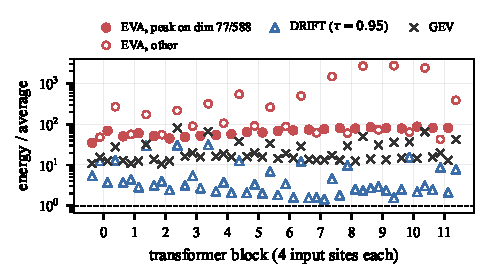
\includegraphics[width=\columnwidth]{figs/fig_outliers.pdf}
\caption{Input energy along each module's leading initial direction, relative
to an average direction (log scale; RoBERTa-base, ChemProt). One point per input
site: $W_Q$, $W_K$ and $W_V$ read the same block input. Filled: EVA's leading
direction peaks on outlier dimension $77$ or $588$; hollow circles: the
attention-output and feed-forward hidden inputs, which are not in the
hidden-state basis. Open triangles: \method{} after deflation; crosses: GEV.}
\label{fig:outliers}
\end{figure}

For most RoBERTa-base modules, the leading principal direction of the input
covariance is one of the backbone's two known outlier dimensions rather than a
direction of biomedical meaning (Fig.~\ref{fig:outliers}). In the modules that
read the hidden state ($W_Q$, $W_K$ and $W_V$, which share the block input, and
the feed-forward up-projection), the leading direction peaks on dimension $588$
or $77$, the outlier dimensions identified for RoBERTa-base
in~\cite{kovaleva2021bertbusters,puccetti2022outliers}. This happens at all $24$
distinct hidden-state inputs on ChemProt and at $23$ of $24$ on RCT-20k and HoC.
Dimension $588$ dominates on ChemProt, and dimension $77$ on HoC. These
directions carry a median $56$--$71\times$ the input energy of an average
direction. The other inputs are no safer. The leading directions of the
attention-output inputs carry a median $50$--$63\times$, and those of the
feed-forward hidden activations a median $254$--$592\times$ and up to
$2{,}748\times$, and over all $72$ modules the median is $59$--$73\times$. (This
ratio of the leading to the mean eigenvalue is the spectral counterpart of a
small participation ratio, in which one direction holds a large
share of the variance.) An adapter whose input-side factor points along such a
direction sees input energy one to three orders of magnitude larger than a
randomly initialised one. A learning rate that is comfortable for LoRA therefore
becomes a very large effective step: in the terms of~\cite{lee2026lrmatters},
curvature rises and the usable learning rate falls. This matches several
observations. First, EVA fails on HoC, where single-seed tuning selected LoRA's
rate for it (Section~\ref{sec:main}). Second, it selects a rate one grid step
below LoRA's on ChemProt and RCT-20k (Appendix~\ref{app:lr}). Third, the account
explains its behaviour at low rank, where the fixed scale $\alpha/r$ is largest.
At ranks $1$ and $2$ it collapses to the constant prediction already at
$3\times10^{-4}$, whereas LoRA, whitened EVA and \method{} still train at
$10^{-3}$, and at $10^{-4}$ its rank-$1$ adapter reaches $78.2\pm2.0$ with the
best dev epoch the last one in every seed (a three-epoch probe at that rate had
not yet left the constant prediction, so it trains late rather than never).
Finally, EVA recovers under whitening, which shrinks these rows.

The general-domain reference carries the same outlier dimensions, which are a
property of the backbone and not of biomedical text, so the reference subspace
absorbs them and deflation removes them. Averaged over the
$768$-dimensional inputs, \method{}'s leading drift direction puts a weight of
$0.009$--$0.017$ on dimension $588$ (against $0.18$--$0.46$ for EVA) and carries
a median of only $1.5$--$2.7\times$ average energy. What the reference removes
first is therefore not ``general English'' in a linguistic sense, as our
motivating argument assumed, but the backbone's own idiosyncratic high-energy
dimensions.

\noindent\textbf{The reference corpus matters only through the backbone.} To
test how much of this is linguistic, we replace WikiText with news articles,
with WikiText whose word order is shuffled within each passage, or with
uniformly random tokens. In every case the reference subspace still absorbs the
outlier dimensions. At $\tau = 0.95$ no leading drift direction peaks on
dimension $77$ or $588$ at any of the $24$ hidden-state inputs, and the leading
directions carry a median $3$--$4\times$ the energy of an average direction with
news or shuffled text and $13$--$15\times$ with random tokens, against
$1.5$--$2.7\times$ with WikiText and $59$--$73\times$ without deflation.
Accuracy follows none of these differences (Table~\ref{tab:ablation}, three
seeds). On ChemProt, \method{} reaches $82.0$, $83.1$ and $82.8$ with the news,
shuffled and random-token references, against $82.3$ with WikiText. On HoC it
reaches $77.8$ and $78.4$ with news and random tokens, against WikiText's
$73.2$, which includes \method{}'s failed seed. No reference differs
significantly from WikiText ($p \ge 0.07$). The shuffled reference's gain over
LoRA on ChemProt ($+0.6$, $p = 0.0007$ uncorrected) rested on three nearly
identical paired differences, the case in which a $t$-test with two degrees of
freedom is least reliable, so we ran seeds $4$ and $5$ of every reference
control. Over five seeds the gain shrinks to $+0.4$ ($p = 0.05$ uncorrected; $p
= 0.24$ after Holm correction over the five reference-versus-LoRA comparisons),
the other references are within $0.2$ points of LoRA, and none of the ten HoC
runs with a replaced reference fails, against one of \method{}'s five with
WikiText. A reference made of random tokens is thus as good as real text: what
the contrast contributes is the backbone's outlier structure, which any input
exposes, not knowledge of general English.

\noindent\textbf{The exact contrast gives the same outcome.} The exact ratio
criterion behaves like its two approximations (Section~\ref{sec:family}). GEV's
leading directions avoid the outlier dimensions at all $24$ hidden-state inputs
and carry a median $8$--$15\times$ average energy (Fig.~\ref{fig:outliers}).
Tuned on its own ($10^{-3}$, $10^{-4}$ and $3\times10^{-4}$), GEV reaches
$82.4$, $83.9$ and $77.6$ on ChemProt, RCT-20k and HoC. This is within $0.3$
points of LoRA on every task ($p \ge 0.72$), with no failed run in fp16, although
one of its three fp32 HoC seeds collapses (Section~\ref{sec:main}), as its
higher initial energy predicts. EVA's own rank-unit rule, under which
feed-forward rank costs no more of the budget than attention rank, spends
$1.26$M (ChemProt) and $1.29$M (HoC) parameters instead of $1.33$M and reaches
$81.9\pm0.5$ and $78.4\pm1.1$ at EVA's rate. On ChemProt this is level with
budget-matched EVA ($+0.1$, $p = 0.87$). The rule fails none of its three HoC
seeds, including seed $2$, on which budget-matched EVA fails. Since fp16
failures are not reproducible from run to run, however, three seeds cannot show
that the rule itself is more stable.

\begin{figure}[t]
\centering
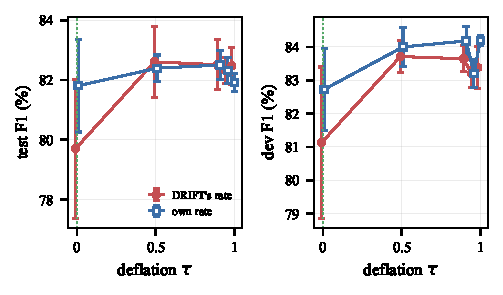
\includegraphics[width=0.9\columnwidth]{figs/fig_tau.pdf}
\caption{Effect of the deflation level $\tau$ on ChemProt (mean$\pm$s.d., three
seeds; test F1 left, best dev F1 right), at \method{}'s learning rate (filled)
and at the rate selected for each level (open). At $\tau = 0$ nothing is deflated
and \method{} coincides with EVA. $\tau = 0.95$ was fixed before any experiment,
so the sweep is descriptive.}
\label{fig:tau}
\end{figure}

\noindent\textbf{Removing the high-energy directions restores most of the
stability but not accuracy.} Without deflation ($\tau = 0$, i.e.\ EVA's
initialisation and allocation) and at \method{}'s learning rate, the method
reaches $79.7\pm2.3$ on ChemProt, whereas any $\tau \in [0.5, 0.99]$ gives
$82.3$--$82.6$ with a standard deviation of $0.4$--$1.2$ (Fig.~\ref{fig:tau}).
At the rate selected for each level, which for $\tau = 0$ is EVA's own, the gap
shrinks to at most $0.7$ points ($\tau = 0$: $81.8\pm1.5$; $\tau \ge 0.5$:
$81.9$--$82.5$ with standard deviations of $0.3$--$0.5$). The robust effect is
the collapse of the scatter rather than a gain in the mean. The curve is flat
from $\tau = 0.5$ onward at either rate, so deflating even half of the
reference energy removes what matters. Whitening achieves the same without a
reference corpus, by rescaling the directions instead of removing them. Yet no
member of the family carries accuracy past LoRA. Whitened EVA, \method{} and GEV
are within $0.5$ points of LoRA on ChemProt and RCT-20k and below it on HoC
(Tables~\ref{tab:main} and~\ref{tab:ablation}).

\subsection{RQ3: allocation or initialisation?}
\label{sec:ablation}

\IfFileExists{tab_ablation.tex}{\begin{table}[t]
\centering
\caption{Ablation (test F1, mean$\pm$s.d.; seeds $1$--$3$ throughout, so the LoRA and \method{} rows differ from the five-seed values of Table~\ref{tab:main}; $1.33$M adapter parameters except EVA's rank-unit rule, which spends $1.26$--$1.29$M). Over five seeds the reference rows give ChemProt 82.3, 82.9, 82.6; HoC 78.0, 77.8 (Section~\ref{sec:outliers}). Upper block: only the allocation rule and the initialisation change, at \method{}'s learning rate. Lower block: the generalised-eigenvector contrast (own rate), EVA with its own budget rule (EVA's rate), and \method{} with its WikiText reference replaced. --: not run.}
\label{tab:ablation}
\footnotesize
\setlength{\tabcolsep}{2.5pt}
\begin{tabular}{lccc}
\toprule
Variant & ChemProt & RCT-20k & HoC \\
\midrule
LoRA (uniform rank, random init) & 82.5\textsubscript{$\pm$\,0.3} & 83.9\textsubscript{$\pm$\,0.2} & 77.9\textsubscript{$\pm$\,1.3} \\
Rank allocation only (random init) & 82.1\textsubscript{$\pm$\,0.3} & 83.9\textsubscript{$\pm$\,0.1} & 65.0\textsubscript{$\pm$\,25.1} \\
Drift init only (uniform rank) & 82.9\textsubscript{$\pm$\,0.9} & 83.9\textsubscript{$\pm$\,0.2} & 78.7\textsubscript{$\pm$\,1.1} \\
Random orthonormal init, drift ranks & 82.3\textsubscript{$\pm$\,1.0} & -- & -- \\
No deflation ($\tau{=}0$), \method{}'s rate & 79.7\textsubscript{$\pm$\,2.3} & -- & -- \\
Absolute (unnormalised) drift score & 82.4\textsubscript{$\pm$\,0.6} & -- & -- \\
\method{} (full) & 82.3\textsubscript{$\pm$\,0.4} & 84.0\textsubscript{$\pm$\,0.1} & 73.2\textsubscript{$\pm$\,10.2} \\
\midrule
GEV init (uniform rank) & 82.4\textsubscript{$\pm$\,0.6} & 83.9\textsubscript{$\pm$\,0.1} & 77.6\textsubscript{$\pm$\,2.2} \\
EVA, rank-unit budget (its own rule) & 81.9\textsubscript{$\pm$\,0.5} & -- & 78.4\textsubscript{$\pm$\,1.1} \\
\method{}, news reference & 82.0\textsubscript{$\pm$\,0.2} & -- & 77.8\textsubscript{$\pm$\,1.9} \\
\method{}, word-shuffled reference & 83.1\textsubscript{$\pm$\,0.3} & -- & -- \\
\method{}, random-token reference & 82.8\textsubscript{$\pm$\,0.4} & -- & 78.4\textsubscript{$\pm$\,0.8} \\
\bottomrule
\end{tabular}
\end{table}
}{}

Table~\ref{tab:ablation} factorises the design space. \method{} changes two
things at once, namely which modules get rank and which subspace each adapter
starts in, so we vary the two independently on all three tasks. On ChemProt we
also add a random-orthonormal initialisation, which separates the \emph{choice}
of subspace from the mere \emph{scale} of an orthonormal initialisation. That
scale differs from LoRA's Kaiming-uniform default and would otherwise be a
confound.

\noindent\textbf{Allocation does not help, and initialisation is neutral to
positive.} Combining \method{}'s rank allocation with LoRA's random
initialisation scores lower than uniform LoRA in every seed on ChemProt
($-0.3$, $p = 0.03$ uncorrected; like the other nominal results, suggestive
only). It is level on RCT-20k ($+0.03$) and destabilising on HoC, where one of
its three seeds fails ($65.0\pm25.1$). \method{}'s initialisation with uniform
ranks is the best low-rank configuration in the upper block on ChemProt
($82.9\pm0.9$), though not significantly better than LoRA ($p = 0.46$). On
RCT-20k and HoC it is level with LoRA ($+0.04$ and $+0.8$, $p \ge 0.41$), with
no failed run. Replacing the drift subspace with a random orthonormal one under
the same ranks leaves the mean unchanged ($82.3$) and doubles the spread, so the
orthonormal scale is not a confound. The unnormalised score changes nothing
either. Allocation is thus the half of the method that costs stability, while
initialisation is the half that is free.

\noindent\textbf{Why allocation has little to work with.} The drift ratio
$\rho_m = \tr(\widetilde{\Sigma}_m)/\tr(\Sigma^{D}_m)$ is small, and most of it
is set by $\tau$ itself. If target and reference shared their geometry exactly,
a fraction $1-\tau$ of the target variance would fall outside the reference
subspace by construction. Averaged over the $48$ distinct input sites, the
excess over $1-\tau$ is only $2.5$ (ChemProt), $2.2$ (RCT-20k) and $1.4$ (HoC)
points of variance at $\tau = 0.95$ ($\rho_m = 7.5$, $7.2$ and $6.4\%$), and
$6.4$/$5.0$/$4.9$ and $0.75$/$0.56$/$0.37$ points at $\tau = 0.5$ and
$\tau = 0.99$. In other words, biomedical text largely reuses the geometry of
general English. The ordering is the same at every $\tau$ and matches lexical
distance from general text, with ChemProt, dense with chemical and protein
names, drifting most. Drift is highest in the first four blocks and roughly flat
beyond them, which is consistent with domain shift entering as unfamiliar
terminology at the lexical end of the network. Because the differences between
sites and tasks amount to a few points of variance, allocation driven by them
has little to exploit. A divergence that does not depend on $\tau$ tells the
same story (Appendix~\ref{app:div}). In CORAL distance, each task's input
covariances sit at $10$--$15$ times the floor between two disjoint halves of
WikiText ($1.17$ for ChemProt, $1.10$ for the clinical notes
of Section~\ref{sec:clinical}, $0.88$ for RCT-20k, $0.76$ for HoC, against
$0.08$). They follow the same order as the drift ratio, and the Bures and
log-det divergences agree. The scale reflects what a corpus is rather than how
useful it is as a reference: news text sits closer to WikiText ($0.92$) and
uniformly random tokens further away ($1.06$) than two of the tasks, yet both
work equally well as references (Section~\ref{sec:outliers}).

The resulting allocations differ visibly. Under a \emph{parameter} budget, an
attention rank unit costs $d^{\mathrm{in}}+d^{\mathrm{out}} = 1{,}536$
parameters against $3{,}840$ for a feed-forward one, so both methods buy cheap
attention capacity first. This is a property of budgeting rather than of either
criterion. Where the two methods differ is in depth. \method{} holds the
attention projections of the first five blocks at the cap ($38\%$ of modules at
the cap, against $18\%$ for EVA) and withdraws rank from blocks $7$--$10$,
driving their feed-forward down-projections to zero. The fact that this visibly
different allocation yields the same accuracy as uniform rank
(Table~\ref{tab:ablation}) is the clearest evidence that, at this budget,
allocation is not where the accuracy lies.

\subsection{RQ3: where should the adapter go?}
\label{sec:placement}

\IfFileExists{tab_placement.tex}{\begin{table}[t]
\centering
\caption{Adapter placement with LoRA, each configuration at its own tuned learning rate (test F1, mean$\pm$s.d., seeds $1$--$3$; Table~\ref{tab:main} reports five seeds for the methods that have them). Rank 14 on the feed-forward matrices spends about the all-module rank-8 budget; rank 4 on all modules about the feed-forward rank-8 budget. \method{} rows use \method{}'s rate. Two of three seeds fail in the feed-forward rank-14 HoC cell at its selected rate; at the rate a three-seed dev mean selects, all three train and it reaches 77.0$\pm$4.1 (Section~\ref{sec:placement}).}
\label{tab:placement}
\footnotesize
\setlength{\tabcolsep}{3pt}
\begin{tabular}{lrrccc}
\toprule
Placement & $r$ & Params & ChemProt & RCT-20k & HoC \\
\midrule
All modules & 8 & 1.33M & 82.5\textsubscript{$\pm$\,0.3} & 83.9\textsubscript{$\pm$\,0.2} & 77.9\textsubscript{$\pm$\,1.3} \\
All modules & 4 & 0.66M & 82.6\textsubscript{$\pm$\,0.5} & 83.5\textsubscript{$\pm$\,0.5} & 78.7\textsubscript{$\pm$\,1.0} \\
Feed-forward only & 8 & 0.74M & 83.4\textsubscript{$\pm$\,0.9} & 83.7\textsubscript{$\pm$\,0.2} & 78.0\textsubscript{$\pm$\,1.4} \\
Feed-forward only & 14 & 1.29M & 82.8\textsubscript{$\pm$\,0.8} & 83.6\textsubscript{$\pm$\,0.4} & 35.0\textsubscript{$\pm$\,35.9} \\
Attention only & 8 & 0.59M & 82.3\textsubscript{$\pm$\,0.5} & 83.9\textsubscript{$\pm$\,0.1} & 77.9\textsubscript{$\pm$\,3.6} \\
\midrule
\method{}, feed-forward only & 8 & 0.74M & 82.8\textsubscript{$\pm$\,0.3} & 83.8\textsubscript{$\pm$\,0.3} & 75.6\textsubscript{$\pm$\,7.8} \\
\method{}, attention only & 8 & 0.59M & 81.2\textsubscript{$\pm$\,0.8} & 83.7\textsubscript{$\pm$\,0.1} & 78.2\textsubscript{$\pm$\,1.5} \\
\bottomrule
\end{tabular}
\end{table}
}{}

Allocation moves rank between modules that all carry an adapter, whereas
placement decides which modules carry one at all. Adapting only the feed-forward
matrices at rank $8$ spends $0.74$M parameters instead of $1.33$M, so a
comparison with all-module rank $8$ confounds placement with budget. This is the
introduction's warning that a matched rank is not a matched budget, in reverse.
The placement study (Table~\ref{tab:placement}) therefore compares each
placement with the other at its budget, on all three tasks, with every
configuration tuned on its own. The pairs are feed-forward-only rank $14$
($1.29$M) against all-module rank $8$ ($1.33$M), and all-module rank $4$
($0.66$M) against feed-forward-only rank $8$ ($0.74$M). The second pair also
tests the alternative explanation that feed-forward-only LoRA wins merely by
having fewer parameters to fit on small data.

\noindent\textbf{At matched budgets.} Neither pair shows a reliable difference.
Against all-module rank $8$, feed-forward-only rank $14$ is $+0.3$ on ChemProt
($p = 0.52$) and $-0.2$ on RCT-20k ($p = 0.53$). On HoC, two of its three seeds
never leave the constant prediction at its selected rate of $10^{-3}$, so that
cell settles nothing until the rate is chosen differently (next paragraph).
Against feed-forward-only rank $8$, all-module rank $4$ is $-0.8$ on
ChemProt ($p = 0.10$), $-0.2$ on RCT-20k ($p = 0.65$) and $+0.7$ on HoC
($p = 0.07$). The lead of feed-forward-only rank $8$ over all-module rank $8$ on
ChemProt ($+0.9$, $p = 0.32$) is therefore not a placement effect that survives
budget matching. Nor are fewer parameters an advantage: all-module rank $4$
($0.66$M) differs from all-module rank $8$ by $+0.1$, $-0.4$ and $+0.8$ points
($p \ge 0.34$), and attention-only rank $8$ ($0.59$M) by at most $0.2$. At this
budget and below it, capacity is not what limits accuracy, and a larger budget
helps only on HoC (Section~\ref{sec:scale}).

\noindent\textbf{Repairing the uninformative HoC cell.} A cell in which two of
three seeds never train supports no comparison at all, so we asked separately
what causes the failures and what a stricter rule would have selected. Precision
explains part of it, but not all. When rerun in fp32 at the same rate, one of
the two failed seeds recovers ($77.3$ and $78.1$ against a third still at
$14.3$). This places the configuration between the fp16 failures that fp32
removes completely and EVA's, which it does not remove at all
(Section~\ref{sec:main}). The selection rule accounts for the rest. Averaged
over the three seeds, the dev score is $35.3$ at the selected $10^{-3}$ and
$80.7$ at $3\times10^{-4}$, so choosing the rate by the multi-seed mean takes
the lower one, where all three seeds train and the test score is $77.0\pm4.1$.
The upward budget-matched comparison therefore rests on that rate rather than on
fp32, and it reaches the same place. Feed-forward-only rank $14$ is $0.9$ points
below all-module rank $8$ ($p = 0.78$) and $1.0$ below feed-forward-only rank
$8$. Placement buys nothing at a matched budget on HoC either. What the cell
adds is a third case, after EVA and AdaLoRA, in which single-seed selection
lands on a rate the configuration cannot reliably train at.

\noindent\textbf{Relation to prior work.} He et al.~\cite{he2022unified} found
that feed-forward modification uses added parameters more effectively than
attention modification, on larger backbones and mostly on generation tasks. We
do not find this with matched budgets, separately tuned learning rates and small
biomedical encoders. Feed-forward-only LoRA is never reliably better than
all-module LoRA at the same budget, and at rank $14$ it is the least stable
configuration on HoC, where it needs a multi-seed learning rate to train at all.
Adapting only attention matches all-module LoRA on every task with less than
half its parameters, and \method{} placed on one module type is never
significantly better than LoRA placed there (it trails on ChemProt with
attention only, $-1.1$, $p = 0.23$, and fails one HoC seed with feed-forward
only). Reallocating the budget between modules, which is what every allocation
method optimises, moves accuracy no more than this coarse choice does, and at
this budget neither moves it measurably.

\subsection{RQ4: budget, scale and architecture}
\label{sec:scale}

\IfFileExists{figs/fig_budget.pdf}{%
\begin{figure}[t]
\centering
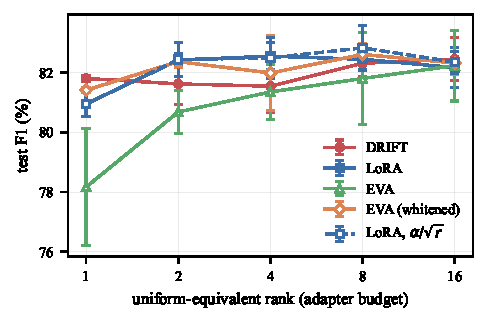
\includegraphics[width=0.9\columnwidth]{figs/fig_budget.pdf}
\caption{Test micro-F1 against adapter budget (uniform-equivalent rank) on
ChemProt, mean$\pm$s.d.\ over three seeds, every (method, budget) pair at its own
tuned learning rate (Appendix~\ref{app:lr}).}
\label{fig:budget}
\end{figure}}{}

\IfFileExists{tab_ladder.tex}{\begin{table}[t]
\centering
\caption{Backbone ladder on ChemProt (test micro-F1, mean$\pm$s.d., three seeds): the BERT miniatures share one vocabulary and pretraining recipe. Each method runs at the learning rate tuned on that backbone's dev set; the last column keeps EVA at the rate tuned for it on RoBERTa-base.}
\label{tab:ladder}
\footnotesize
\setlength{\tabcolsep}{1.4pt}
\begin{tabular}{lccccc}
\toprule
BERT & LoRA & EVA & \shortstack{EVA\\(whitened)} & \method{} & \shortstack{EVA\\(RoBERTa's rate)} \\
\midrule
Tiny (4.4M) & 60.9\textsubscript{$\pm$\,1.9} & 58.3\textsubscript{$\pm$\,1.1} & 59.3\textsubscript{$\pm$\,1.2} & \textbf{61.2\textsubscript{$\pm$\,1.8}} & 47.5\textsubscript{$\pm$\,3.4} \\
Mini (11.2M) & \textbf{70.8\textsubscript{$\pm$\,0.9}} & 68.4\textsubscript{$\pm$\,2.1} & 69.1\textsubscript{$\pm$\,0.8} & 70.1\textsubscript{$\pm$\,0.9} & 63.9\textsubscript{$\pm$\,0.8} \\
Small (28.8M) & \textbf{76.1\textsubscript{$\pm$\,0.7}} & 74.4\textsubscript{$\pm$\,0.4} & 74.6\textsubscript{$\pm$\,0.4} & 74.8\textsubscript{$\pm$\,0.7} & 71.1\textsubscript{$\pm$\,0.7} \\
Medium (41.4M) & \textbf{77.6\textsubscript{$\pm$\,0.7}} & 76.5\textsubscript{$\pm$\,1.3} & 76.7\textsubscript{$\pm$\,0.5} & 76.6\textsubscript{$\pm$\,1.1} & 74.9\textsubscript{$\pm$\,0.9} \\
Base (110.1M) & 79.2\textsubscript{$\pm$\,0.9} & 79.2\textsubscript{$\pm$\,1.3} & 79.8\textsubscript{$\pm$\,0.4} & \textbf{80.5\textsubscript{$\pm$\,0.5}} & 79.2\textsubscript{$\pm$\,1.3} \\
\bottomrule
\end{tabular}
\end{table}
}{}

\noindent\textbf{Budget.} Across budgets from rank $1$ to $16$ on ChemProt
(Fig.~\ref{fig:budget}), with the learning rate tuned at every budget, LoRA,
\method{} and whitened EVA stay within $1.0$ points of each other at every
budget, and LoRA is flat from rank $2$ ($82.4$) to rank $16$. EVA trails at the
smallest budgets ($-2.8$ and $-1.7$ against LoRA at ranks $1$ and $2$; $p = 0.10$
and $0.03$ uncorrected) and catches up by rank $16$. Tuning keeps its rate at
$10^{-4}$ up to rank $8$, half a decade to a decade below the other methods'
rates. Where the budget binds hardest, at rank $1$, \method{} has the
best mean ($81.8\pm0.1$ against LoRA's $81.0\pm0.4$; $+0.9$, $p = 0.04$
uncorrected, not significant after Holm correction over the sweep's twelve
comparisons with LoRA). This is the one place in our study where allocation
might have room to help. We keep the scale $\alpha/r$, as EVA does, rather than
rsLoRA's $\alpha/\sqrt{r}$~\cite{kalajdzievski2023rslora}. Under Adam, changing
the scale multiplies every update of $sBA$ by the same factor, and per-rank
tuning of the learning rate absorbs this to first order. The dashed curve in
Fig.~\ref{fig:budget} tests this argument. LoRA with $\alpha/\sqrt{r}$, tuned at
every rank, stays within $0.4$ points of LoRA with $\alpha/r$ at every budget
(largest difference $+0.4$ at rank $8$, $p = 0.58$), and at rank $1$, where the
two scales coincide, the two runs reproduce each other exactly. Per-rank tuning
thus absorbs the change of scale.

\noindent\textbf{Budget on the other tasks.} Whether the ranking changes with the
budget is not only a question for ChemProt. At $0.5\%$ (rank $4$) and $2\%$
(rank $16$) on RCT-20k and HoC, with every method and budget tuned on its own
(Appendix~\ref{app:budgetx}), the results match the picture that
Table~\ref{tab:main} gives at rank $8$. On RCT-20k the four methods lie within
$0.6$ points of each other at every budget, with whitened EVA and \method{}
marginally above LoRA at rank $4$ ($+0.4$, $p \ge 0.25$), while on HoC LoRA has
the best mean at all three budgets. There, EVA trails it by $1.4$ at rank $4$
and $2.5$ at rank $16$, whitened EVA by $1.3$ at both, and \method{} loses a
seed at rank $4$ ($61.3\pm29.1$) and trails by $5.4$ at rank $16$. Two
differences reach $p < 0.05$ uncorrected, both of them losses to LoRA (EVA at
rank $16$ on RCT-20k, $-0.5$; \method{} at rank $16$ on HoC, $-5.4$), and
neither survives Holm correction over the table's twelve comparisons. HoC is
also the one place where the budget itself matters. LoRA at rank $16$ beats LoRA
at rank $8$ by $2.4$ points ($p = 0.05$ uncorrected), while rank $4$ is level
with rank $8$ on all three tasks. So where a larger budget helps, allocating it
differently still does not.

\noindent\textbf{Model scale.} Table~\ref{tab:ladder} tests the prediction from
Section~I that allocation should matter more as the backbone shrinks, now with
every method tuned on every backbone. The prediction is not borne out. LoRA has
the best mean on BERT-Mini, -Small and -Medium, and \method{} on BERT-Tiny
($+0.3$, $p = 0.89$) and BERT-Base ($+1.3$, $p = 0.03$ uncorrected). The latter
is the largest gain over LoRA in the ladder but not significant after Holm
correction over its twenty comparisons with LoRA. At their own tuned rates, EVA
trails LoRA by $0.0$ to $2.5$ points and whitened EVA by at most $1.8$, none
significantly. The last column keeps EVA at the rate tuned for it on
RoBERTa-base ($10^{-4}$), as our first version of this study did. EVA then
falls further behind as the backbone shrinks: it is level on BERT-Base but
$2.7$, $4.9$, $6.9$ and $13.4$ points behind the tuned LoRA from BERT-Medium
down to BERT-Tiny. The one difference in the ladder
that survives correction is this column's loss on BERT-Mini. Most of that
deficit was caused by the inherited learning rate and not by the
initialisation, which is the clearest single illustration of why a rate tuned
for one backbone is not a neutral choice for another. After per-backbone tuning,
what remains is a small EVA deficit that grows as the backbone shrinks ($0.0$ on
BERT-Base, $1.2$ on BERT-Medium, $1.7$ on BERT-Small, $2.5$ on BERT-Mini and
BERT-Tiny).

\noindent\textbf{Profile noise on small backbones.} A narrow backbone profiled
from $1{,}024$ sequences might simply get noisy directions. We therefore
profiled BERT-Tiny from all $4{,}169$ ChemProt training sentences and all
$3{,}227$ WikiText passages (four and three times the standard profile, and all
the text these corpora have). This changes EVA, whitened EVA and \method{} by
$+0.7$, $+1.3$ and $-0.9$ points, none significantly ($p \ge 0.20$). EVA
remains $1.8$ points behind LoRA, so its shortfall on the smallest backbone is
not mainly estimation noise in the profile.

\noindent\textbf{Outlier dimensions across the ladder.} Profiling the BERT
miniatures shows that the mechanism of Section~\ref{sec:outliers} is not
specific to RoBERTa, but also that it does not explain EVA's deficit. If we count
distinct inputs to the hidden-state modules ($W_Q$, $W_K$ and $W_V$ share one),
a single dimension hosts EVA's leading direction at $13$ of $24$ inputs on
BERT-Base, in every layer, and at $11$ of $16$ on BERT-Medium, compared with
$23$ of $24$ on RoBERTa-base. The pattern weakens to $5$ of $8$ on BERT-Mini and
$3$ of $8$ on BERT-Small, and no dimension recurs across BERT-Tiny's four
inputs. The energy excess shrinks as well. EVA's leading directions carry a
median $59\times$ the energy of an average direction on BERT-Base, then
$40\times$, $36\times$, $20\times$ and $11\times$ down to BERT-Tiny, because
their share of the variance stays near $7$--$8\%$ at the hidden-state inputs
while the width falls from $768$ to $128$ (deflation cuts them to
$1.6$--$4.9\times$). On its own, the mechanism therefore predicts milder
instability on small backbones, not stronger, and the ladder agrees. At its
tuned rate EVA fails no run on any BERT miniature, and its seed standard
deviation ($0.4$--$2.1$ points) is of the order of LoRA's ($0.7$--$1.9$). EVA's
small deficit, which grows as the backbone shrinks while the energy excess
falls, must therefore have another cause, which these experiments do not
isolate.

\IfFileExists{tab_decoder.tex}{\begin{table}[t]
\centering
\caption{Decoder SLM: SmolLM2-360M (test F1, mean$\pm$s.d., three seeds), each method at its own tuned learning rate (rate above the score).}
\label{tab:decoder}
\footnotesize
\setlength{\tabcolsep}{3pt}
\begin{tabular}{lcc}
\toprule
Method & ChemProt & HoC \\
\midrule
LoRA & \shortstack{$10^{-3}$\\\textbf{83.9\textsubscript{$\pm$\,0.5}}} & \shortstack{$10^{-3}$\\\textbf{80.9\textsubscript{$\pm$\,0.8}}} \\
EVA (budget-matched) & \shortstack{$3{\times}10^{-4}$\\82.2\textsubscript{$\pm$\,3.6}} & \shortstack{$10^{-3}$\\74.6\textsubscript{$\pm$\,5.5}} \\
EVA (whitened) & \shortstack{$10^{-3}$\\83.1\textsubscript{$\pm$\,1.4}} & \shortstack{$10^{-3}$\\80.5\textsubscript{$\pm$\,0.3}} \\
\method{} & \shortstack{$10^{-3}$\\83.4\textsubscript{$\pm$\,1.9}} & \shortstack{$10^{-3}$\\80.3\textsubscript{$\pm$\,0.9}} \\
\bottomrule
\end{tabular}
\end{table}
}{}

\noindent\textbf{A decoder SLM.} SmolLM2-360M, a decoder-only SLM, reproduces
the pattern seen on RoBERTa on ChemProt (Table~\ref{tab:decoder}), with every
method tuned on its own dev set under the same protocol. Its outlier signature
is the strongest we measured. Dimension $40$ hosts EVA's leading direction at
$41$ of the $64$ hidden-state inputs, in layers $1$--$25$ of $32$. This is
consistent with the massive activations reported for LLMs, which also sit in
fixed dimensions of the middle layers~\cite{sun2024massive}. EVA's leading
directions carry a median $125\times$ the energy of an average direction
($6.3\times$ after deflation). Tuning again places EVA's learning rate one grid
step below LoRA's ($3\times10^{-4}$ against $10^{-3}$, just as $10^{-4}$ against
$3\times10^{-4}$ on RoBERTa-base's ChemProt). Whitened EVA and \method{}, whose
initial directions carry little excess energy, select LoRA's rate or a higher
one on ChemProt on both backbones. This is what the curvature account of
Section~\ref{sec:outliers} predicts, with a lower usable rate for EVA alone. No
method beats LoRA ($83.9\pm0.5$), and EVA is again the least stable
($82.2\pm3.6$, one seed at $78.1$). On HoC, where the encoder's failures
occurred and $512$-token documents require a batch of $8$, all four methods
train without a failed run and tuning gives all of them $10^{-3}$. LoRA reaches
$80.9\pm0.8$, whitened EVA $80.5\pm0.3$ and \method{} $80.3\pm0.9$, while EVA is
again the least stable at $74.6\pm5.5$, with seeds at $80.6$, $73.3$ and $69.9$
($-6.3$ against LoRA, $p = 0.22$). In fp16 the decoder thus repeats the
encoder's pattern, with the same ordering and instability concentrated in EVA,
but the cause differs. In two of EVA's three seeds the per-epoch logs show the
fp16 loss scale collapsing to zero, with no gradient reaching the adapter from
the fifth epoch on, so their scores come from checkpoints of the second and
third epochs, which stay above our failure threshold. Rerun in fp32
(Section~\ref{sec:setup}) at the same rate and from the same profile, EVA trains
in every seed without a non-finite step, although its gradient norm before
clipping still reaches $291$, against at most $12.8$ for LoRA. It scores
$79.8\pm1.7$, level with LoRA's $80.7\pm1.5$ in fp32 ($-0.9$, $p = 0.66$), and
precision leaves LoRA itself unchanged ($-0.2$, $p = 0.91$). On the decoder,
EVA's instability is fp16 overflow, not the early collapse it shows on
RoBERTa-base, and removing it again adds no accuracy.

\subsection{Clinical notes}
\label{sec:clinical}

\IfFileExists{tab_clinical.tex}{\begin{table}[t]
\centering
\caption{Clinical notes (MTSamples, 12 specialties; test micro- and macro-F1, mean$\pm$s.d.\ over three seeds). Each method runs at the rate tuned on the clinical dev set; the reference rows use \method{}'s rate. $\Delta$: paired difference to LoRA in micro-F1. Failed: as in Table~\ref{tab:main}.}
\label{tab:clinical}
\footnotesize
\setlength{\tabcolsep}{2.5pt}
\begin{tabular}{lcccc}
\toprule
Method & Micro-F1 & Macro-F1 & $\Delta$ ($p$) & Failed \\
\midrule
LoRA & 84.6\textsubscript{$\pm$\,1.0} & 84.3\textsubscript{$\pm$\,1.8} & -- & 0/3 \\
EVA (budget-matched) & 83.5\textsubscript{$\pm$\,0.2} & 81.5\textsubscript{$\pm$\,1.2} & -1.1 (0.20) & 0/3 \\
EVA (whitened) & 83.4\textsubscript{$\pm$\,0.6} & 82.7\textsubscript{$\pm$\,1.0} & -1.2 (0.13) & 0/3 \\
\method{} & 84.5\textsubscript{$\pm$\,0.2} & 83.4\textsubscript{$\pm$\,0.8} & -0.1 (0.86) & 0/3 \\
\midrule
\method{}, news reference & 84.4\textsubscript{$\pm$\,1.4} & 83.3\textsubscript{$\pm$\,1.2} & -0.2 (0.74) & 0/3 \\
\method{}, random-token reference & 85.1\textsubscript{$\pm$\,0.6} & 84.4\textsubscript{$\pm$\,0.4} & +0.4 (0.66) & 0/3 \\
\bottomrule
\end{tabular}
\end{table}
}{}

PubMed abstracts are stylistically close to WikiText, but clinical notes, with
their abbreviations, templated sections and dictation style, are not. To test
whether our findings survive the shift our deployment motivation implies, we add
a clinical task: classifying transcribed clinical notes from
MTSamples~\cite{mtsamples} by medical specialty. The public release lists many
notes under both a specialty and a document type (e.g.\ ``Surgery'' or
``Discharge Summary''). We drop the document-type and catch-all labels, drop the
notes that remain listed under two specialties, and keep the $12$ specialties
with at least $70$ notes ($1{,}972$ notes), split $70/15/15$ within each
specialty and truncated to $512$ tokens. LoRA, EVA, whitened EVA and
\method{} are each tuned on the clinical dev set, and \method{} also runs with
the news and random-token references (Table~\ref{tab:clinical}).

Both the mechanism and the conclusions carry over. EVA's leading directions peak
on dimension $77$ or $588$ at $21$ of the $24$ hidden-state inputs of the
clinical profile and carry a median $57\times$ the energy of an average
direction, compared with $24$ of $24$ and $73\times$ on ChemProt. Deflation
leaves one such input and a median of $4.0\times$. The drift ratio matches
ChemProt's, with an excess over $1-\tau$ of $2.6$ points at $\tau = 0.95$,
against $2.5$. Tuning selects $10^{-4}$ for all four methods, and no run fails.
LoRA is again unbeaten---$84.6$ micro-F1 ($84.3$ macro) against \method{}'s
$84.5$ ($-0.1$, $p = 0.86$), EVA's $83.5$ ($-1.1$, $p = 0.20$) and whitened
EVA's $83.4$ ($-1.2$, $p = 0.13$). The random-token reference gives the best
mean in the table ($85.1$, $+0.4$ over LoRA, $p = 0.66$) and the news reference
$84.4$, so the reference corpus does not matter on clinical text either.
Clinical style changes none of the quantities we measured, and the backbone's
outliers dominate its activations as they do on PubMed abstracts.

\subsection{Cost of profiling}
\label{sec:cost}

Profiling consists of two forward passes, one eigendecomposition of each
reference covariance $\Sigma^{G}_m$, and one eigendecomposition of each projected
target covariance per value of $\tau$. On one NVIDIA T4, the GPU used for every
training run, the two forward passes over
$1{,}024$ reference and $1{,}024$ target sequences take $28$--$35$\,s at the
short sequence lengths of ChemProt and RCT-20k and $99$\,s at HoC's $512$
tokens. The spectral step takes $45$--$47$\,s for one $\tau$ and $136$--$143$\,s
for five. This is nearly independent of the task, because the cost is set by
the module dimensions ($768$ and $3{,}072$) rather than by the amount of text.
The step runs on the CPU in double precision and could be moved to the GPU. In
total, profiling at one $\tau$ costs $42$--$47\%$ of a single LoRA training run
on the same task and GPU. That is cheap, but not negligible, and it is not free
relative to the accuracy it buys at this budget. The reference pass can be
reused, since $\Sigma^{G}_m$ depends only on the backbone, and a deployment that
adapts one model to many domains pays for it only once. Because the adapter
merges into the base weights after training, the inference cost is identical to
that of LoRA and of the unadapted backbone.

\section{Discussion: Evaluating Adapter Allocation}
\label{sec:discussion}

Inference cost does not separate the methods we compare. Every low-rank adapter
merges into the backbone after training, so the costs that differ are training
and profiling time, and the only question is whether profiling buys accuracy.
Our results do not say that adapter capacity is irrelevant, since at rank $1$ it
does bind. What they say is that, for small encoders at a budget of about $1\%$,
where the capacity goes (across modules or across module types) matters less
than how each configuration is trained, that is, the learning rate selected for
it and the energy of its initial directions. Fig.~\ref{fig:protocol} condenses
these lessons into a protocol, and we explain the reasons below.

\begin{figure}[t]
\centering
\fbox{\begin{minipage}{0.94\columnwidth}
\small
\textbf{A protocol for evaluating adapter allocation}
\begin{enumerate}\setlength{\itemsep}{1pt}\setlength{\leftmargin}{1.2em}
\item \emph{Budget in parameters.} Match adapter parameters, not total rank,
      and report the parameters actually spent (head excluded).
\item \emph{Tune every configuration.} Select the learning rate on the dev set
      separately for every method, backbone, budget and placement, and extend
      each grid until the selection is interior.
\item \emph{Seeds and failures.} Use at least five seeds on small tasks. Report
      medians and failed runs next to means, rerun failures in fp32 to separate
      numerics from method, and correct for multiple comparisons.
\item \emph{Energy check.} Before training a data-derived initialisation,
      compute each initial direction's energy relative to an average direction
      (target forward pass plus one leading eigenvector per module). On
      RoBERTa-base and SmolLM2-360M, medians of $59$--$125\times$ coincided with
      failed or unstable runs and $1$--$15\times$ with stable training; on the BERT ladder
      $20$--$59\times$ trained stably at tuned rates. Read a high median as a
      warning to lower the rate, whiten or deflate---not as a verdict.
\item \emph{Check that the budget binds.} Before trying allocation, run LoRA at
      half the budget and at other placements of the same budget. If nothing
      changes, allocation has nothing to exploit. Neither check needs profiling.
\end{enumerate}
\end{minipage}}
\caption{A protocol for evaluating adapter allocation, distilled from
Section~\ref{sec:results}.}
\label{fig:protocol}
\end{figure}

\noindent\textbf{Match parameters, and tune every configuration.} A rank unit
costs $1{,}536$ parameters in an attention projection of RoBERTa-base and
$3{,}840$ in a feed-forward matrix, so equal total rank is not an equal budget.
AdaLoRA, pruned to the total rank of uniform rank $8$, ends at up to $1.43$M
parameters rather than $1.33$M. Methods also favour different learning
rates~\cite{lee2026lrmatters}, and so do backbones and budgets. Without these
controls, a new allocation rule can gain simply by spending more parameters, or
by being compared at a learning rate chosen for another configuration. At the
rate selected on RoBERTa-base, EVA fell $13.4$ points behind the tuned LoRA on
BERT-Tiny, and at the rate tuned on BERT-Tiny itself only $2.5$.

\noindent\textbf{Report spread and failures, not only means.} On HoC the methods
are separated by failed runs rather than by accuracy, and a single run can land
on either side. Two fp16 runs of \method{} with identical settings reached $82.5$
and $66.2$ dev F1. In fp32, the failures of PiSSA, DoRA and \method{} vanished
while EVA's became universal, so the same count of failed runs can mean
numerical noise for one method and a genuine instability for another. One
method can even fall on both sides: EVA's instability on the decoder vanished in
fp32 (Section~\ref{sec:scale}). Medians,
failure counts, an fp32 check and a multiplicity correction make such
differences visible, instead of averaging them into a mean that describes no
run.

\noindent\textbf{Check the energy of a data-derived initialisation.} On a
backbone with outlier dimensions, these dimensions dominate the principal
directions of the activations. Computing the energy of each initial direction
relative to an average one (Fig.~\ref{fig:outliers}) costs only the target half
of the profiling pass ($10$--$63$\,s here) and a leading eigenvector per module.
EVA's medians were $59$--$73\times$ on RoBERTa-base, where it failed runs, and
$125\times$ on SmolLM2-360M, where it failed no run but was the least stable
method in fp16, against $1$--$15\times$ for the initialisations that largely
restored stability (whitened EVA, $1\times$ by
construction; \method{} with any of our four references; GEV). The residual
risk follows the same scale. GEV, the highest of these at $8$--$15\times$, is
the one that still lost a run. The check is a warning rather than a verdict. On
the BERT ladder, initialisations at $20$--$59\times$ trained stably at tuned
rates, including EVA's $59\times$ on BERT-Base. Recurring outlier dimensions
also appear in BERT-Base, BERT-Medium and SmolLM2-360M, so the diagnostic is not
specific to RoBERTa, but it is not decisive on its own either.

\noindent\textbf{Check whether the budget binds.} An allocation rule can only
help where capacity is scarce, and at $1\%$ of RoBERTa-base it usually is not.
All-module LoRA at half the budget and attention-only LoRA at less than half
match the full budget on all three tasks, and on ChemProt rank $2$, a quarter of
it, is within $0.1$ points. Where the budget does bind, the answer is the same.
At rank $1$ on ChemProt, \method{} has its only nominal gain of the budget
sweep, and on HoC, where doubling the budget to $2\%$ gains LoRA $2.4$ points,
no allocation rule beats LoRA at that budget either. A budget sweep and a
placement comparison need no profiling, whereas profiling costs almost half a
training run (Section~\ref{sec:cost}).

\noindent\textbf{What this means for defaults and for their authors.} PEFT
libraries ship the choices our baseline uses (adapters on all linear maps,
$s = \alpha/r$, Kaiming-uniform $A$ and $B = 0$), and our results support them
as defaults for small encoders, with two amendments. First, report the
parameters an adapter actually spends, since placement and allocation change
them far more than they change accuracy here. Second, make data-derived
initialisations report the energy of their directions. For EVA, the
configuration we test differs from the published one in its budget unit, so
Section~\ref{sec:outliers} also reports the published rank-unit rule. That rule
spends slightly fewer parameters, matches budget-matched EVA's accuracy and
failed none of its three HoC seeds, so our conclusions about EVA do not hinge on
the budget unit. Our decoder results use last-token classification, and
practitioners who use decoders generatively face a different objective, about
which we make no claim.

\noindent\textbf{Deployment.} Everything here runs on a single commodity GPU
with a frozen, shared backbone, which keeps sensitive data inside an
institution. If anything, the move towards small on-premise models
that this study supports is privacy-positive.

\section{Limitations}

\noindent\textbf{Input-side profiling cannot separate $W_Q$, $W_K$ and $W_V$.}
These three projections consume the same block input, so they share a
covariance matrix and receive identical drift scores. As a result, \method{}
resolves four distinct sites per block rather than six. Distinguishing them
requires an output-side signal, which costs a backward pass and would give up
the gradient-free property. Our allocation routine already accepts an optional
per-module weight for exactly this purpose, and we leave a hybrid variant to
future work.

\noindent\textbf{The reference corpus is a proxy.}
Assumption (A) is stated with respect to the pretraining distribution, which is
not public for most checkpoints. We substitute WikiText-103, a general-domain
corpus that is clearly not RoBERTa's training set, so (A) holds only
approximately. We tested three substitutes for it (Section~\ref{sec:outliers}),
and each, random tokens included, served as well.
We did not test references closer to the pretraining mix.

\noindent\textbf{Statistical power and selection.}
Three to five seeds detect only large differences. Our conclusion that no
method beats LoRA therefore rules out gains of the size typically claimed for
adaptive allocation (a point or more), but not small ones. The runs behind
Table~\ref{tab:main} did not store per-example predictions, so its intervals
come from a replication of every parameter-efficient run in it
(Appendix~\ref{app:ci}), and Appendix~\ref{app:seeds} lists every seed. Learning
rates are selected on one seed, which on HoC puts several methods near the edge
of stability. Selecting EVA's rate by the mean over three fp32 seeds instead
(Section~\ref{sec:main}) removes its failures but leaves it $2.7$ points below
LoRA. The controls of Table~\ref{tab:ablation} inherit their parent
configuration's rate (Section~\ref{sec:setup}). Differences inside the table's
upper block, the $-0.3$ of allocation alone among them, therefore
compare variants at \method{}'s rate rather than at each variant's own, and are
suggestive for that reason too. We did not re-select after observing test
results.

\noindent\textbf{Clinical text and first-order shift.}
Our motivation is clinical deployment, but apart from the MTSamples task our
data are public PubMed text, which is stylistically much closer to WikiText than
clinical notes are. The MTSamples notes are sample reports published as
reference and training material for medical transcriptionists, and they are not
records from an electronic health record. They carry no de-identification tokens
and little of the noise of real notes, so they test clinical style rather than
clinical deployment. All profile-based methods here also centre their inputs,
so a mean shift between domains, which is plausibly a large part of the shift
towards clinical text, is invisible to them by construction.

\noindent\textbf{Scope.}
We study the classification of biomedical and clinical text. The full budget
sweep, the $\tau$ sweep and the ladder use ChemProt only. The placement study
and the allocation/initialisation factorisation cover all three benchmarks, the
reference controls and the decoder cover ChemProt and HoC, the two further
budgets ($0.5\%$ and $2\%$) cover RCT-20k and HoC, and the clinical task covers
only the four methods on which the analysis turns. Architectures without
pronounced outlier dimensions may not show EVA's instability at all. Larger
decoders, generative formulations and other specialised domains remain
untested. HoC has only 371 test documents, so its confidence intervals are wide
(Appendix~\ref{app:ci}).

\noindent\textbf{One profiling pass per task.}
The drift profile depends on the target corpus, so a new domain requires a fresh
(cheap) profiling pass. Where many tasks share one domain, the profile can be
reused, but we have not measured how much this loses.

\section{Conclusion}

Activation-guided allocation asks where the target distribution's variance is
largest. On RoBERTa-base, for most modules, the answer is one of two outlier
dimensions of the backbone, and adapters initialised there are fragile.
Whitening those directions, deflating them with a general-domain reference
(\method{}), or taking the generalised eigenvectors of the target and reference
covariances restores most of the stability without labels, gradients or
inference cost. But under a matched parameter budget, with every configuration
tuned on its own, no such fix and no allocation rule we tested outperformed
uniform LoRA on three biomedical benchmarks, a clinical task or a decoder SLM.
Rank allocation alone slightly hurt, adapter placement changed nothing reliable
at a matched budget, and half the budget was enough. On smaller backbones the
learning rate tuned for each backbone, not any allocation rule, decided how far
EVA trailed LoRA.

We believe this is the right baseline for the field to report against.
Improvements claimed for activation-aware allocation should be measured at
matched parameters, against a separately tuned LoRA, at learning rates tuned for
the backbone, budget and placement in question, over enough seeds to reveal
their failures, and checked for the stability of their initialisation. Natural
next steps are to test the outlier mechanism in larger decoders, generative
tasks and real clinical records, and to ask whether a cheap output-side signal
can make allocation matter where input geometry alone does not.

\bibliographystyle{IEEEtran}
\bibliography{refs}

\clearpage
% One column for the appendix: its tables are wide, and in two-column mode each
% one takes a float page of its own (round-2 NEW-7).
\onecolumn
\appendices

\section{Learning-rate selection}
\label{app:lr}
For every configuration from which a conclusion is drawn, Table~\ref{tab:lr}
lists the learning rate selected on the dev set (seed $1$) and the range of the
grid from which it was chosen.

\IfFileExists{tab_lr.tex}{\begin{table*}[!ht]
\centering
\caption{Learning-rate selection (dev set, seed 1) for all 119 tuned configurations. Each grid starts from the listed first values and is extended one step past whichever edge holds the best score until the selection is interior; no selection lies on an edge of its final grid.}
\label{tab:lr}
\scriptsize
\setlength{\tabcolsep}{3pt}
\begin{tabular}{llll}
\toprule
Configuration & Selected & Configuration & Selected \\
\midrule
RoBERTa-base, ChemProt, \method{} & 3e-4 [1e-5, 1e-3] & RoBERTa-base, ChemProt, LoRA, $r{=}16$ & 1e-3 [1e-4, 3e-3] \\
RoBERTa-base, ChemProt, LoRA & 3e-4 [1e-4, 1e-3] & RoBERTa-base, ChemProt, EVA, $r{=}16$ & 3e-4 [3e-5, 1e-3] \\
RoBERTa-base, ChemProt, EVA & 1e-4 [1e-5, 3e-4] & RoBERTa-base, ChemProt, EVA (whitened), $r{=}16$ & 3e-4 [1e-4, 1e-3] \\
RoBERTa-base, ChemProt, EVA (whitened) & 1e-3 [1e-5, 3e-3] & BERT-Tiny, ChemProt, \method{} & 1e-3 [1e-4, 3e-3] \\
RoBERTa-base, ChemProt, AdaLoRA & 3e-3 [1e-4, 1e-2] & BERT-Tiny, ChemProt, LoRA & 3e-3 [1e-4, 1e-2] \\
RoBERTa-base, ChemProt, Full fine-tuning & 5e-5 [1e-5, 1e-4] & BERT-Tiny, ChemProt, EVA & 1e-3 [1e-4, 3e-3] \\
RoBERTa-base, ChemProt, BitFit & 1e-3 [3e-4, 3e-3] & BERT-Tiny, ChemProt, EVA (whitened) & 3e-3 [1e-4, 1e-2] \\
RoBERTa-base, ChemProt, Linear probe & 5e-3 [1e-3, 2e-2] & BERT-Mini, ChemProt, \method{} & 1e-3 [1e-4, 3e-3] \\
RoBERTa-base, ChemProt, PiSSA & 3e-4 [1e-4, 1e-3] & BERT-Mini, ChemProt, LoRA & 1e-3 [1e-4, 3e-3] \\
RoBERTa-base, ChemProt, DoRA & 1e-3 [1e-4, 3e-3] & BERT-Mini, ChemProt, EVA & 1e-3 [1e-4, 3e-3] \\
RoBERTa-base, RCT-20k, \method{} & 1e-4 [1e-5, 3e-4] & BERT-Mini, ChemProt, EVA (whitened) & 1e-3 [1e-4, 3e-3] \\
RoBERTa-base, RCT-20k, LoRA & 3e-4 [1e-4, 1e-3] & BERT-Small, ChemProt, \method{} & 3e-4 [1e-4, 1e-3] \\
RoBERTa-base, RCT-20k, EVA & 1e-4 [1e-5, 3e-4] & BERT-Small, ChemProt, LoRA & 1e-3 [1e-4, 3e-3] \\
RoBERTa-base, RCT-20k, EVA (whitened) & 1e-4 [1e-5, 3e-4] & BERT-Small, ChemProt, EVA & 1e-3 [1e-4, 3e-3] \\
RoBERTa-base, RCT-20k, AdaLoRA & 3e-3 [1e-4, 1e-2] & BERT-Small, ChemProt, EVA (whitened) & 1e-3 [1e-4, 3e-3] \\
RoBERTa-base, RCT-20k, Full fine-tuning & 3e-5 [1e-5, 5e-5] & BERT-Medium, ChemProt, \method{} & 3e-4 [1e-4, 1e-3] \\
RoBERTa-base, RCT-20k, BitFit & 3e-3 [3e-4, 1e-2] & BERT-Medium, ChemProt, LoRA & 1e-3 [1e-4, 3e-3] \\
RoBERTa-base, RCT-20k, Linear probe & 2e-2 [1e-3, 5e-2] & BERT-Medium, ChemProt, EVA & 3e-4 [1e-4, 1e-3] \\
RoBERTa-base, RCT-20k, PiSSA & 1e-4 [3e-5, 3e-4] & BERT-Medium, ChemProt, EVA (whitened) & 3e-4 [1e-4, 1e-3] \\
RoBERTa-base, RCT-20k, DoRA & 1e-4 [3e-5, 3e-4] & BERT-Base, ChemProt, \method{} & 1e-3 [1e-4, 3e-3] \\
RoBERTa-base, HoC, \method{} & 3e-4 [1e-5, 1e-3] & BERT-Base, ChemProt, LoRA & 3e-4 [1e-4, 1e-3] \\
RoBERTa-base, HoC, LoRA & 3e-4 [1e-4, 1e-3] & BERT-Base, ChemProt, EVA & 1e-4 [3e-5, 1e-3] \\
RoBERTa-base, HoC, EVA & 3e-4 [1e-5, 1e-3] & BERT-Base, ChemProt, EVA (whitened) & 1e-3 [1e-4, 3e-3] \\
RoBERTa-base, HoC, EVA (whitened) & 1e-4 [1e-5, 3e-4] & SmolLM2-360M, HoC, LoRA & 1e-3 [3e-4, 3e-3] \\
RoBERTa-base, HoC, AdaLoRA & 3e-3 [1e-4, 1e-2] & SmolLM2-360M, HoC, EVA & 1e-3 [1e-4, 3e-3] \\
RoBERTa-base, HoC, Full fine-tuning & 5e-5 [1e-5, 1e-4] & SmolLM2-360M, HoC, EVA (whitened) & 1e-3 [3e-4, 3e-3] \\
RoBERTa-base, HoC, BitFit & 1e-3 [3e-4, 3e-3] & SmolLM2-360M, HoC, \method{} & 1e-3 [3e-4, 3e-3] \\
RoBERTa-base, HoC, Linear probe & 2e-2 [1e-3, 5e-2] & RoBERTa-base, ChemProt, LoRA, $r{=}1$, rsLoRA scale & 1e-3 [1e-4, 3e-3] \\
RoBERTa-base, HoC, PiSSA & 3e-4 [1e-4, 1e-3] & RoBERTa-base, ChemProt, LoRA, $r{=}2$, rsLoRA scale & 3e-4 [1e-4, 1e-3] \\
RoBERTa-base, HoC, DoRA & 3e-4 [1e-4, 1e-3] & RoBERTa-base, ChemProt, LoRA, $r{=}4$, rsLoRA scale & 3e-4 [1e-4, 1e-3] \\
RoBERTa-base, ChemProt, LoRA, attention only & 1e-3 [1e-4, 3e-3] & RoBERTa-base, ChemProt, LoRA, rsLoRA scale & 3e-4 [1e-4, 1e-3] \\
RoBERTa-base, ChemProt, LoRA, FFN only & 1e-3 [1e-4, 3e-3] & RoBERTa-base, ChemProt, LoRA, $r{=}16$, rsLoRA scale & 3e-4 [1e-4, 1e-3] \\
RoBERTa-base, ChemProt, LoRA, FFN only, $r{=}14$ & 1e-3 [1e-4, 3e-3] & RoBERTa-base, RCT-20k, \method{}, $r{=}4$ & 3e-4 [1e-4, 1e-3] \\
RoBERTa-base, ChemProt, LoRA, $r{=}4$ & 3e-4 [1e-4, 1e-3] & RoBERTa-base, RCT-20k, EVA, $r{=}4$ & 1e-4 [3e-5, 3e-4] \\
RoBERTa-base, RCT-20k, LoRA, attention only & 3e-4 [1e-4, 1e-3] & RoBERTa-base, RCT-20k, EVA (whitened), $r{=}4$ & 3e-4 [1e-4, 1e-3] \\
RoBERTa-base, RCT-20k, LoRA, FFN only & 3e-4 [1e-4, 1e-3] & RoBERTa-base, RCT-20k, \method{}, $r{=}16$ & 1e-4 [3e-5, 1e-3] \\
RoBERTa-base, RCT-20k, LoRA, FFN only, $r{=}14$ & 1e-3 [1e-4, 3e-3] & RoBERTa-base, RCT-20k, LoRA, $r{=}16$ & 3e-4 [1e-4, 1e-3] \\
RoBERTa-base, RCT-20k, LoRA, $r{=}4$ & 1e-3 [1e-4, 3e-3] & RoBERTa-base, RCT-20k, EVA, $r{=}16$ & 3e-4 [3e-5, 1e-3] \\
RoBERTa-base, HoC, LoRA, attention only & 3e-4 [1e-4, 1e-3] & RoBERTa-base, RCT-20k, EVA (whitened), $r{=}16$ & 3e-4 [1e-4, 1e-3] \\
RoBERTa-base, HoC, LoRA, FFN only & 1e-3 [1e-4, 3e-3] & RoBERTa-base, HoC, \method{}, $r{=}4$ & 3e-4 [1e-4, 1e-3] \\
RoBERTa-base, HoC, LoRA, FFN only, $r{=}14$ & 1e-3 [1e-4, 3e-3] & RoBERTa-base, HoC, EVA, $r{=}4$ & 1e-4 [3e-5, 3e-4] \\
RoBERTa-base, HoC, LoRA, $r{=}4$ & 3e-4 [1e-4, 1e-3] & RoBERTa-base, HoC, EVA (whitened), $r{=}4$ & 1e-4 [3e-5, 1e-3] \\
RoBERTa-base, ChemProt, GEV & 1e-3 [1e-4, 3e-3] & RoBERTa-base, HoC, \method{}, $r{=}16$ & 1e-4 [3e-5, 1e-3] \\
RoBERTa-base, RCT-20k, GEV & 1e-4 [3e-5, 1e-3] & RoBERTa-base, HoC, LoRA, $r{=}16$ & 3e-4 [1e-4, 1e-3] \\
RoBERTa-base, HoC, GEV & 3e-4 [1e-4, 1e-3] & RoBERTa-base, HoC, EVA, $r{=}16$ & 1e-4 [3e-5, 3e-4] \\
RoBERTa-base, ChemProt, \method{}, $\tau{=}0.5$ & 1e-3 [1e-4, 3e-3] & RoBERTa-base, HoC, EVA (whitened), $r{=}16$ & 3e-4 [1e-4, 1e-3] \\
RoBERTa-base, ChemProt, \method{}, $\tau{=}0.9$ & 1e-3 [1e-4, 3e-3] & RoBERTa-base, ChemProt, LoRA, linear head & 3e-4 [1e-4, 1e-3] \\
RoBERTa-base, ChemProt, \method{}, $\tau{=}0.99$ & 1e-3 [1e-4, 3e-3] & RoBERTa-base, ChemProt, EVA, linear head & 1e-4 [3e-5, 3e-4] \\
RoBERTa-base, ChemProt, \method{}, $r{=}1$ & 3e-4 [1e-4, 1e-3] & RoBERTa-base, ChemProt, EVA (whitened), linear head & 1e-3 [1e-4, 3e-3] \\
RoBERTa-base, ChemProt, LoRA, $r{=}1$ & 1e-3 [1e-4, 3e-3] & RoBERTa-base, ChemProt, \method{}, linear head & 1e-3 [1e-4, 3e-3] \\
RoBERTa-base, ChemProt, EVA, $r{=}1$ & 1e-4 [3e-5, 3e-4] & RoBERTa-base, ChemProt, BitFit, linear head & 1e-3 [3e-4, 3e-3] \\
RoBERTa-base, ChemProt, EVA (whitened), $r{=}1$ & 1e-3 [1e-4, 3e-3] & RoBERTa-base, MTSamples, LoRA & 1e-4 [3e-5, 1e-3] \\
RoBERTa-base, ChemProt, \method{}, $r{=}2$ & 1e-3 [1e-4, 3e-3] & RoBERTa-base, MTSamples, EVA & 1e-4 [3e-5, 3e-4] \\
RoBERTa-base, ChemProt, LoRA, $r{=}2$ & 1e-3 [1e-4, 3e-3] & RoBERTa-base, MTSamples, EVA (whitened) & 1e-4 [3e-5, 1e-3] \\
RoBERTa-base, ChemProt, EVA, $r{=}2$ & 1e-4 [3e-5, 3e-4] & RoBERTa-base, MTSamples, \method{} & 1e-4 [3e-5, 1e-3] \\
RoBERTa-base, ChemProt, EVA (whitened), $r{=}2$ & 1e-3 [1e-4, 3e-3] & SmolLM2-360M, ChemProt, \method{} & 1e-3 [1e-5, 3e-3] \\
RoBERTa-base, ChemProt, \method{}, $r{=}4$ & 1e-3 [1e-4, 3e-3] & SmolLM2-360M, ChemProt, EVA & 3e-4 [1e-5, 3e-3] \\
RoBERTa-base, ChemProt, EVA, $r{=}4$ & 1e-4 [3e-5, 3e-4] & SmolLM2-360M, ChemProt, EVA (whitened) & 1e-3 [1e-5, 3e-3] \\
RoBERTa-base, ChemProt, EVA (whitened), $r{=}4$ & 1e-3 [1e-4, 3e-3] & SmolLM2-360M, ChemProt, LoRA & 1e-3 [1e-4, 3e-3] \\
RoBERTa-base, ChemProt, \method{}, $r{=}16$ & 1e-3 [1e-4, 3e-3] &  &  \\
\bottomrule
\end{tabular}
\end{table*}
}{}

\section{Per-seed results}
\label{app:seeds}
Table~\ref{tab:seeds} lists the test score of every seed in
Table~\ref{tab:main}.

\IfFileExists{tab_seeds.tex}{\begin{table*}[!ht]
\centering
\caption{Per-seed test scores of Table~\ref{tab:main} (seeds 1, 2, 3 and, for LoRA, EVA, whitened EVA and \method{}, seeds 4 and 5), with the 95\% $t$-interval of the mean over seeds.}
\label{tab:seeds}
\scriptsize
\setlength{\tabcolsep}{2.5pt}
\begin{tabular}{lllllll}
\toprule
Method & ChemProt & 95\% CI & RCT-20k & 95\% CI & HoC & 95\% CI \\
\midrule
Full fine-tuning & 82.1 / 81.9 / 81.3 & [80.7, 82.8] & 84.0 / 84.1 / 83.0 & [82.1, 85.3] & 74.9 / 78.4 / 75.5 & [71.5, 81.0] \\
Linear probe & 49.4 / 48.7 / 49.8 & [47.9, 50.7] & 77.5 / 77.8 / 76.7 & [75.9, 78.7] & 48.5 / 50.9 / 47.0 & [43.9, 53.7] \\
BitFit & 81.4 / 81.4 / 81.2 & [81.0, 81.7] & 84.0 / 83.8 / 83.9 & [83.6, 84.1] & 77.5 / 78.7 / 78.5 & [76.7, 79.8] \\
LoRA & 82.6 / 82.1 / 82.7 / 82.5 / 82.7 & [82.2, 82.8] & 83.6 / 83.9 / 84.1 / 83.4 / 83.7 & [83.4, 84.1] & 76.5 / 78.3 / 78.9 / 76.6 / 79.5 & [76.3, 79.7] \\
DoRA & 81.9 / 82.2 / 83.0 & [80.9, 83.9] & 83.7 / 83.5 / 83.7 & [83.3, 83.9] & 80.5 / 14.3 / 79.1 & [-36.0, 151.9] \\
PiSSA & 82.1 / 82.0 / 83.1 & [80.9, 83.9] & 83.9 / 83.8 / 83.8 & [83.7, 84.0] & 61.5 / 14.3 / 77.8 & [-30.7, 133.1] \\
AdaLoRA & 82.6 / 81.8 / 83.6 & [80.5, 84.9] & 84.3 / 82.0 / 80.7 & [77.8, 86.9] & 79.0 / 77.7 / 77.7 & [76.3, 79.9] \\
EVA (budget-matched) & 82.7 / 80.0 / 82.7 / 80.5 / 81.5 & [80.0, 83.0] & 83.9 / 83.5 / 83.7 / 83.9 / 83.7 & [83.5, 84.0] & 77.5 / 26.2 / 76.5 / 79.0 / 37.8 & [27.9, 90.9] \\
EVA (whitened) & 82.9 / 82.8 / 82.2 / 83.8 / 78.5 & [79.5, 84.6] & 83.9 / 83.8 / 84.0 / 84.0 / 84.1 & [83.8, 84.1] & 78.0 / 77.8 / 76.4 / 78.8 / 75.5 & [75.6, 78.9] \\
\method{} & 82.1 / 82.1 / 82.8 / 82.5 / 82.5 & [82.0, 82.8] & 84.0 / 84.0 / 83.9 / 83.7 / 84.0 & [83.8, 84.1] & 61.4 / 79.0 / 79.3 / 80.0 / 78.7 & [65.8, 85.6] \\
GEV & 81.8 / 82.9 / 82.6 & [81.0, 83.8] & 83.9 / 83.9 / 84.0 & [83.8, 84.0] & 75.2 / 79.4 / 78.3 & [72.2, 83.0] \\
\bottomrule
\end{tabular}
\end{table*}
}{}

\section{Instance-level intervals}
\label{app:ci}
The runs of Table~\ref{tab:main} did not store per-example predictions, so we
repeated every one of them with the same configurations, rates and seeds, this
time storing the predictions, and we bootstrap over seeds and test examples
jointly (Table~\ref{tab:ci}). Paired differences to LoRA resample the same seeds
and examples for both methods. The replicate means also measure run-to-run
variation under fp16. On ChemProt and RCT-20k every replicate reproduces its
Table~\ref{tab:main} run exactly, while on HoC the two differ by $0.5$ to $21$
points. The large values come from seeds that failed in one run and not in the
other (DoRA $+21.1$, PiSSA $+11.8$, EVA $+6.0$, \method{} $+3.3$, against $+1.0$
for LoRA).

\IfFileExists{tab_ci.tex}{\begin{table*}[!ht]
\centering
\caption{Instance-level uncertainty for Table~\ref{tab:main}: a replication of every parameter-efficient run that stores per-example test predictions, with 95\% hierarchical bootstrap intervals (seeds, then test examples, $2{,}000$ replicates). $\Delta$: paired difference to LoRA (same seeds and examples). Rep.: replicate mean minus the Table~I mean (fp16 run-to-run variation).}
\label{tab:ci}
\scriptsize
\setlength{\tabcolsep}{2.5pt}
\begin{tabular}{lccccccccc}
\toprule
 & \multicolumn{3}{c}{ChemProt} & \multicolumn{3}{c}{RCT-20k} & \multicolumn{3}{c}{HoC} \\
Method & Mean [95\% CI] & $\Delta$ vs LoRA [95\% CI] & Rep. & Mean [95\% CI] & $\Delta$ vs LoRA [95\% CI] & Rep. & Mean [95\% CI] & $\Delta$ vs LoRA [95\% CI] & Rep. \\
\midrule
BitFit & 81.3 [80.1, 82.5] & -1.1 [-2.0, -0.2] & +0.0 & 83.9 [82.9, 84.8] & +0.0 [-0.6, +0.6] & +0.0 & 79.5 [76.2, 82.8] & +0.6 [-1.9, +3.3] & +1.3 \\
LoRA & 82.5 [81.3, 83.7] & -- & +0.0 & 83.7 [82.8, 84.6] & -- & +0.0 & 79.0 [75.7, 82.3] & -- & +1.0 \\
DoRA & 82.4 [81.1, 83.6] & -0.1 [-1.0, +0.8] & +0.0 & 83.6 [82.7, 84.5] & -0.2 [-0.7, +0.3] & +0.0 & 79.0 [75.8, 82.1] & +0.1 [-2.5, +2.6] & +21.1 \\
PiSSA & 82.4 [81.1, 83.7] & -0.1 [-0.9, +0.7] & +0.0 & 83.8 [82.9, 84.7] & -0.1 [-0.6, +0.5] & +0.0 & 63.0 [34.6, 80.6] & -15.9 [-45.9, +1.9] & +11.8 \\
AdaLoRA & 82.7 [81.3, 84.1] & +0.2 [-0.7, +1.1] & +0.0 & 82.3 [80.5, 84.2] & -1.5 [-3.4, +0.5] & -0.0 & 78.8 [75.4, 82.0] & -0.1 [-2.8, +2.6] & +0.7 \\
EVA (budget-matched) & 81.5 [80.0, 83.0] & -1.0 [-2.1, +0.0] & +0.0 & 83.7 [82.8, 84.7] & +0.0 [-0.5, +0.6] & +0.0 & 65.4 [39.5, 80.6] & -13.6 [-41.3, +1.3] & +6.0 \\
EVA (whitened) & 82.0 [80.1, 83.9] & -0.5 [-2.5, +1.1] & +0.0 & 84.0 [83.0, 84.8] & +0.2 [-0.2, +0.7] & -0.0 & 77.8 [74.3, 80.9] & -1.2 [-3.4, +0.9] & +0.5 \\
\method{} & 82.4 [81.3, 83.6] & -0.1 [-0.7, +0.5] & +0.0 & 83.9 [83.0, 84.8] & +0.2 [-0.3, +0.7] & +0.0 & 79.0 [75.8, 82.2] & +0.0 [-2.0, +2.1] & +3.3 \\
GEV & 82.4 [81.1, 83.6] & -0.1 [-1.1, +1.0] & +0.0 & 83.9 [83.0, 84.8] & +0.1 [-0.5, +0.6] & +0.0 & 79.7 [76.4, 82.9] & +0.8 [-1.1, +3.0] & +2.1 \\
\bottomrule
\end{tabular}
\end{table*}
}{}

\section{A linear classification head}
\label{app:linhead}
Every method trains RoBERTa's classification head, whose $0.60$M parameters are
shared by all methods and could compress their differences. Replacing the head
with a single linear layer on the first token, and tuning every configuration
again, lowers every method except \method{} by $0.6$--$1.5$ points and changes
no conclusion (Table~\ref{tab:linhead}). LoRA reaches $81.9\pm0.1$, \method{}
$82.7\pm0.7$ ($+0.8$, $p = 0.14$), whitened EVA $81.1\pm0.8$, BitFit
$80.6\pm0.5$ and EVA $80.4\pm0.3$ ($-1.5$, $p = 0.03$ uncorrected).

\IfFileExists{tab_linhead.tex}{\begin{table}[h]
\centering
\caption{ChemProt with the backbone's classification head (Table~\ref{tab:main}, seeds 1--3) and with a single linear head on the first token ($768\times13$), every configuration tuned on its own (test micro-F1, three seeds).}
\label{tab:linhead}
\footnotesize
\begin{tabular}{lcc}
\toprule
Method & \shortstack{RoBERTa head\\($0.60$M)} & \shortstack{Linear head\\($0.01$M)} \\
\midrule
LoRA & 82.5\textsubscript{$\pm$\,0.3} & 81.9\textsubscript{$\pm$\,0.1} \\
EVA (budget-matched) & 81.8\textsubscript{$\pm$\,1.5} & 80.4\textsubscript{$\pm$\,0.3} \\
EVA (whitened) & 82.6\textsubscript{$\pm$\,0.4} & 81.1\textsubscript{$\pm$\,0.8} \\
\method{} & 82.3\textsubscript{$\pm$\,0.4} & 82.7\textsubscript{$\pm$\,0.7} \\
BitFit & 81.3\textsubscript{$\pm$\,0.1} & 80.6\textsubscript{$\pm$\,0.5} \\
\bottomrule
\end{tabular}
\end{table}
}{}

\section{$\tau$-free divergences}
\label{app:div}
Table~\ref{tab:div} gives three divergences between the input covariances of
each corpus and those of WikiText. Unlike the drift ratio, these do not depend
on $\tau$. They are the CORAL distance, the Bures--Wasserstein distance and the
symmetrised log-det (Jeffreys) divergence between trace-normalised covariances,
each averaged over the $48$ distinct input sites. The floor is the divergence
between two disjoint halves of WikiText at the same sequence length.

\IfFileExists{tab_div.tex}{\begin{table}[h]
\centering
\caption{Tau-free divergence of each corpus's input covariances from the WikiText reference (trace-normalised; mean over the $48$ distinct input sites). Floor: a disjoint half of WikiText at the same sequence length. News and random tokens at ChemProt's length.}
\label{tab:div}
\footnotesize
\setlength{\tabcolsep}{3pt}
\begin{tabular}{lccc}
\toprule
Corpus vs.\ WikiText & CORAL & Bures & Jeffreys \\
\midrule
ChemProt & 1.172 & 0.3456 & 0.653 \\
\quad floor (ChemProt length) & 0.076 & 0.0068 & 0.016 \\
News (CNN/DailyMail) & 0.920 & 0.1787 & 0.281 \\
Random tokens & 1.058 & 0.4378 & 0.893 \\
RCT-20k & 0.878 & 0.2306 & 0.411 \\
\quad floor (RCT-20k length) & 0.081 & 0.0079 & 0.019 \\
HoC & 0.763 & 0.2093 & 0.393 \\
\quad floor (HoC length) & 0.075 & 0.0056 & 0.013 \\
MTSamples & 1.105 & 0.2770 & 0.495 \\
\quad floor (MTSamples length) & 0.075 & 0.0056 & 0.013 \\
\bottomrule
\end{tabular}
\end{table}
}{}

\section{Budgets on RCT-20k and HoC}
\label{app:budgetx}
Table~\ref{tab:budgetx} extends the budget comparison of Fig.~\ref{fig:budget}
to RCT-20k and HoC at ranks $4$ and $16$, with every method and budget tuned on
its own. Rank $8$ repeats the configuration of Table~\ref{tab:main} over seeds
$1$--$3$.

\IfFileExists{tab_budgetx.tex}{\begin{table}[h]
\centering
\caption{Adapter budget on RCT-20k and HoC (mean$\pm$s.d., three seeds, every method and budget tuned on its own). Rank $4$, $8$ and $16$ spend $0.53\%$, $1.06\%$ and $2.1\%$ of the backbone.}
\label{tab:budgetx}
\footnotesize
\setlength{\tabcolsep}{2.5pt}
\begin{tabular}{llcccc}
\toprule
Task & $r$ & LoRA & EVA & \shortstack{EVA\\(whitened)} & \method{} \\
\midrule
RCT-20k & 4 & 83.5\textsubscript{$\pm$\,0.5} & 83.8\textsubscript{$\pm$\,0.2} & \textbf{83.9\textsubscript{$\pm$\,0.1}} & \textbf{83.9\textsubscript{$\pm$\,0.4}} \\
 & 8 & 83.9\textsubscript{$\pm$\,0.2} & 83.7\textsubscript{$\pm$\,0.2} & 83.9\textsubscript{$\pm$\,0.1} & \textbf{84.0\textsubscript{$\pm$\,0.1}} \\
 & 16 & 84.0\textsubscript{$\pm$\,0.1} & 83.5\textsubscript{$\pm$\,0.3} & \textbf{84.1\textsubscript{$\pm$\,0.1}} & 83.9\textsubscript{$\pm$\,0.2} \\
\midrule
HoC & 4 & \textbf{78.7\textsubscript{$\pm$\,1.0}} & 77.4\textsubscript{$\pm$\,1.6} & 77.4\textsubscript{$\pm$\,0.6} & 61.3\textsubscript{$\pm$\,29.1} \\
 & 8 & \textbf{77.9\textsubscript{$\pm$\,1.3}} & 60.1\textsubscript{$\pm$\,29.3} & 77.4\textsubscript{$\pm$\,0.9} & 73.2\textsubscript{$\pm$\,10.2} \\
 & 16 & \textbf{80.3\textsubscript{$\pm$\,1.6}} & 77.8\textsubscript{$\pm$\,2.2} & 79.0\textsubscript{$\pm$\,0.5} & 74.9\textsubscript{$\pm$\,0.6} \\
\bottomrule
\end{tabular}
\end{table}
}{}

\end{document}
